% !TEX root = thesis.tex

% Die vorliegende Arbeit stellt mit ihrem Anspruch und Vorhaben eine der Kernaufgaben der Geoinf dar, Probleme der Domain Experts in Bezug auf Datenverarb erfassung auswertung infornmationstechn lösen, effektiv machen

% moving average
% map-reduce
% aggregation
\chapter{Introduction}
	Recent research has highlighted the relevance of lakes to global process such as the carbon cycle \citep{cole2007plumbing}.
	Ecological studies on lakes have historically taken advantage of the “closed system” bounds to delineate a simplified ecosystem, but analyses that are formulated to answer societally relevant questions often must scale this single system science approach to hundreds, thousands, or millions of lakes \citep{downing2006global}.
	Therefore systems must be developed that can aggregate, analyze, and ultimately interpret hydrological data at large scales. Additionally, these analytical systems must be able to easily couple lake features with supporting data that define, for example, catchment properties, local climate, and anthropomorphic stressors.
	These data products are readily available as national coverages that can either be sampled and turned into model parameters, or turned into model drivers if they are time series products.

	This work shall evaluate the existing tools \citep[e.g. \la\fu{https://github.com/GLEON/Lake-Analyzer}, see][]{read2011derivation}), data models and the modeling frameworks used by USGS CIDA\fu{http://cida.usgs.gov/}.
	Modeling runs are based on online data brokers (such as the USGS’s \ac{GDP}\fu{http://cida.usgs.gov/gdp/}) build upon \ac{OGC} standards such as \acrocitep{CSW}{ogc:csw}, \acrocitep{WPS}{ogc:wps}, \acrocitep{WMS}{ogc:wms} and \acrocitep{WCS}{ogc:csw}, but still rely on local algorithms, which comprise functionality for statistical quality assurance and quality control as well as the calculation of various metrics related to the physical state of the lakes (often linked with ecosystem function or disturbance). Building standardized and flexible infrastructure for analyzing foundational data used by domain scientists is an important challenge given legacy and heterogeneous architectures.
	Therefore building on the existing infrastructure and corresponding demands of the use case shall be considered.

	One approach for a scalable system is to move the modeling to a web-based processing framework, which should rely on public and interoperable standards in the given use case.
	Web processing allows to chain data brokers with translators, models, and eventually post-hoc analysis of model runs.
	This chain provides specific information products to the user.
	Considering the amount of data (and future process scaling needs), such an analysis must be conducted in a streaming manner, i.e. the processing should start before the last chunk of data comes in, and the output should also be available in parts before the processing has completely finished to reduce the lag for domain users of the system.
	Existing approaches to this problem shall be critically evaluated.

	This thesis work comprises the evaluation, design and prototypical implementation of a lake analysis chain for live sensor data.
	This includes the evaluation of existing data models (mainly CSV/TSV) and a standardized way to convert existing domain specific applications written in MatLab\fu{http://www.mathworks.de/products/matlab/} into streaming web services (possibly WPS algorithms) in favor of the currently used non standardized web frontend\fu{http://lakeanalyzer.gleon.org/}.

	\paragraph*{Research Questions}
	\begin{itemize}
		\item How can large scale hydrological data be processed in a service-based processing chain?
		\item Do available web-processing interface definitions support a live data streaming scenario, what is missing?
		\item Can real-time data be integrated into the processing chain for a constant (streamed) analysis?
		\item How does the developed architecture perform in practical test with 1000s and 10000s of lake features?
		\item How can continued statistical quality assurance and quality control in the application area of lake ecology be modeled in a web service chain?
		\item Do existing standards (data models and service interfaces for data warehousing, processing and visualization) support a streaming analysis chain? What is missing?
		\item How can spatial dependencies between streamed features be considered?
		\item How can a analysis language commonly used by domain experts (in this case MatLab) be easily deployed in a web based processing chain?
	\end{itemize}

\chapter{\la}
	\la is tool to compute key characteristics of lakes with regards to the lake's thermal stratification and its stability. It analyzes times series data of water temperature measurements obtained using instrumented lake buoys as well as wind speed observations using the lake's bathymetric areas with respect to depth and optional salinity measurements to improve water density calculations. It promotes comparative lake research, which is made possible due to the increased temporal resolution and spatial extent of lake measurements by offering a consistent methodology that can be applied to many types of lakes \citep{read2011derivation}.

	\la allows to predict biological phenomenon (e.g. the likelihood of nutrient upwelling that can cause algal blooms), explain phenological pattern in aquatic organisms, control and monitor the state of a lake as well as to improve the quality of models by comparing their outputs to the physical state of the lake that is computed by the \la.

	Besides a raw data output as \ac{CSV}, the \la features a visualizations of the produces stratification and mixing indices, which can be seen in \cref{fig:la:outputs:1}: Lake Number \citep[see \cref{fig:la:out:Ln,fig:la:out:SLn},][]{imberger1990}, metalimnion extent (see \cref{fig:la:out:metaT,fig:la:out:metaB,fig:la:out:SmetaT,fig:la:out:SmetaB}), Brunt-Väisälä buoyancy frequency (see \cref{fig:la:out:N2,fig:la:out:SN2}), mode-1 vertical seiche period \citep[see \cref{fig:la:out:T1,fig:la:out:ST1},][]{monismith1986}, Wedderburn Number \citep[see \cref{fig:la:out:W,fig:la:out:SW},][]{thompson1980}, thermocline depth (see \cref{fig:la:out:thermD,fig:la:out:SthermD}), $u^{*}$ (wind stress introduced water friction velocity, see \cref{fig:la:out:uSt,fig:la:out:SuSt}) and Schmidt Stability \citep[see \cref{fig:la:out:St},][]{schmidt1928,hutchinson1957,idso1973}. The \la is able to error check and/or down sample input time series and also outputs wind speed (\cref{fig:la:out:wndSpd}) and water temperature (\cref{fig:la:out:wTemp}).

	\def\lafigsize{.497\linewidth}
	\begin{figure}
		\centering
		\begin{subfigure}{\lafigsize}
			\caption{\label{fig:la:out:Ln}Lake Number}
			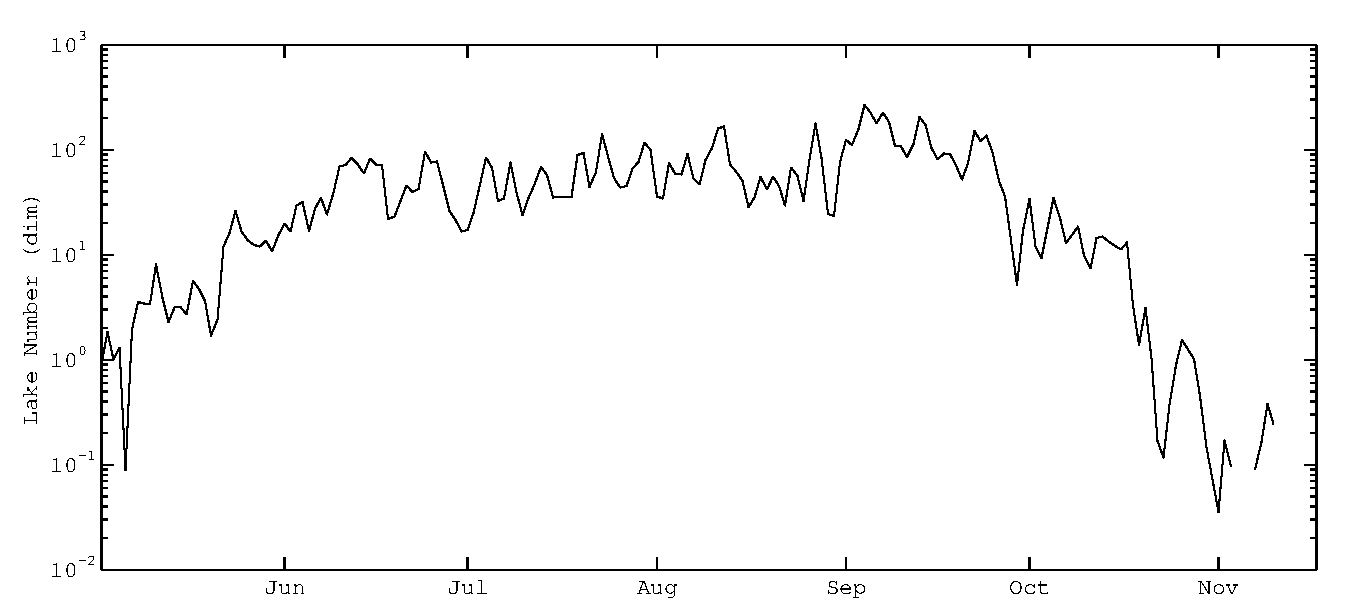
\includegraphics[width=\linewidth]{figures/Sparkling_Ln.pdf}
		\end{subfigure}
		\begin{subfigure}{\lafigsize}
			\caption{\label{fig:la:out:SLn}Seasonal Lake Number}
			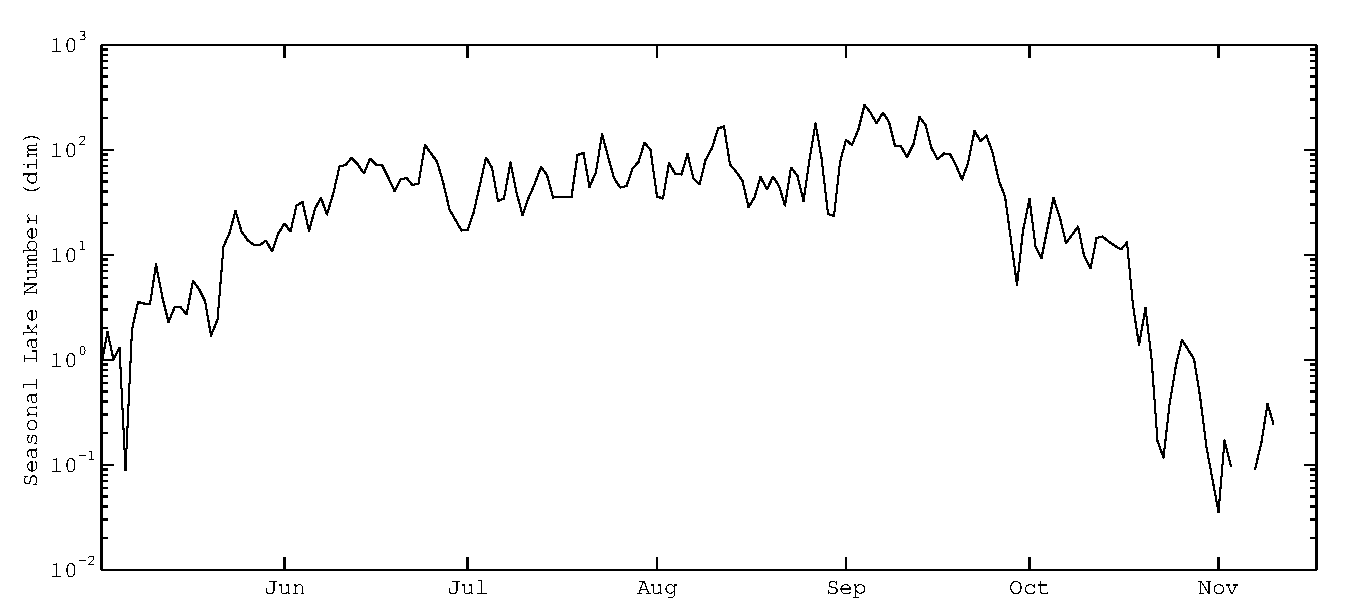
\includegraphics[width=\linewidth]{figures/Sparkling_SLn.pdf}
		\end{subfigure}
		\begin{subfigure}{\lafigsize}
			\caption{\label{fig:la:out:metaT}Metalimnion Top}
			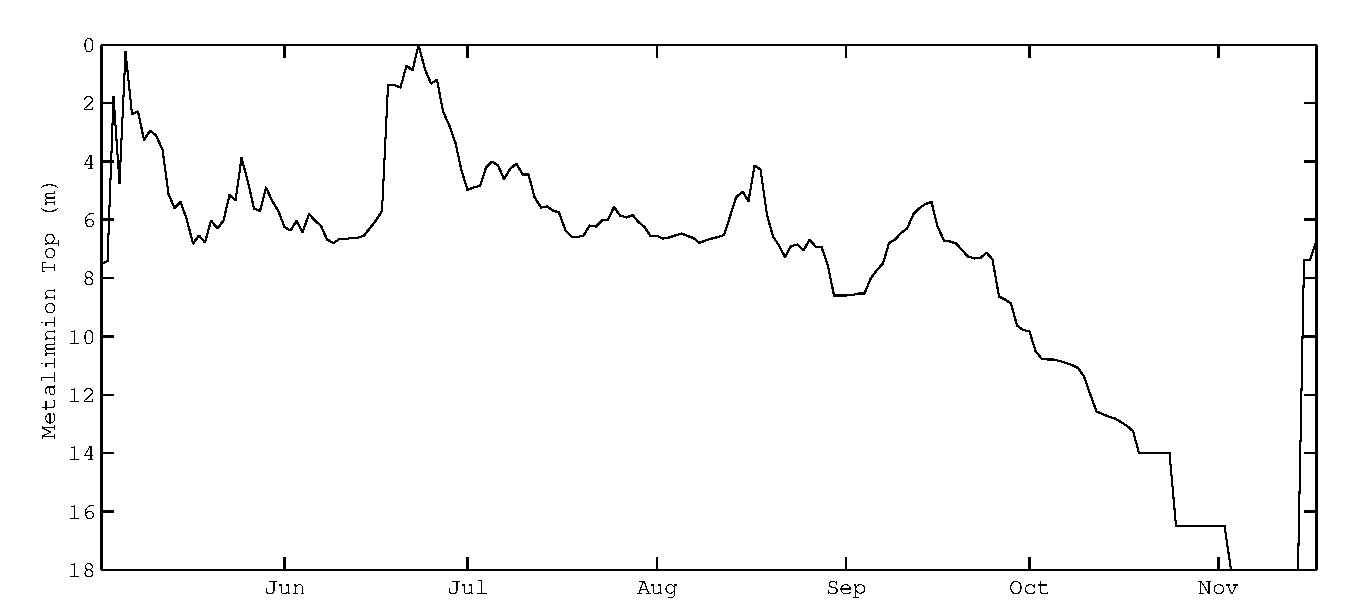
\includegraphics[width=\linewidth]{figures/Sparkling_metaT.pdf}
		\end{subfigure}
		\begin{subfigure}{\lafigsize}
			\caption{\label{fig:la:out:metaB}Metalimnion Bottom}
			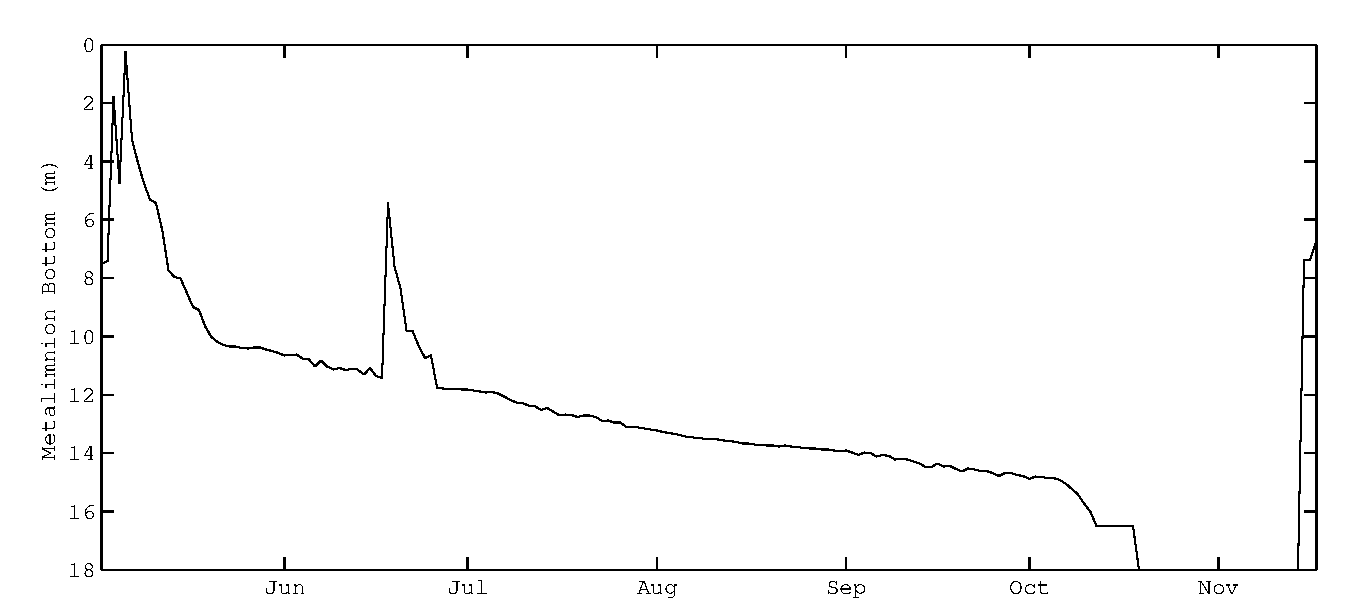
\includegraphics[width=\linewidth]{figures/Sparkling_metaB.pdf}
		\end{subfigure}
		\begin{subfigure}{\lafigsize}
			\caption{\label{fig:la:out:SmetaT}Seasonal Metalimnion Top}
			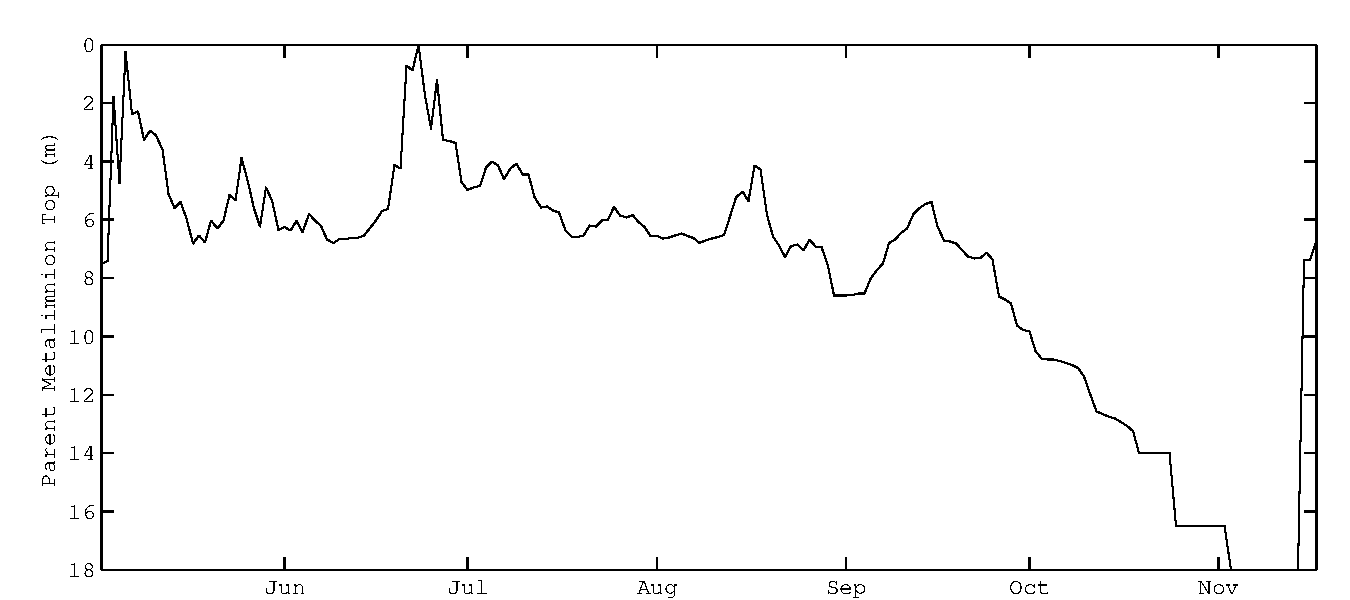
\includegraphics[width=\linewidth]{figures/Sparkling_SmetaT.pdf}
		\end{subfigure}
		\begin{subfigure}{\lafigsize}
			\caption{\label{fig:la:out:SmetaB}Seasonal Metalimnion Bottom}
			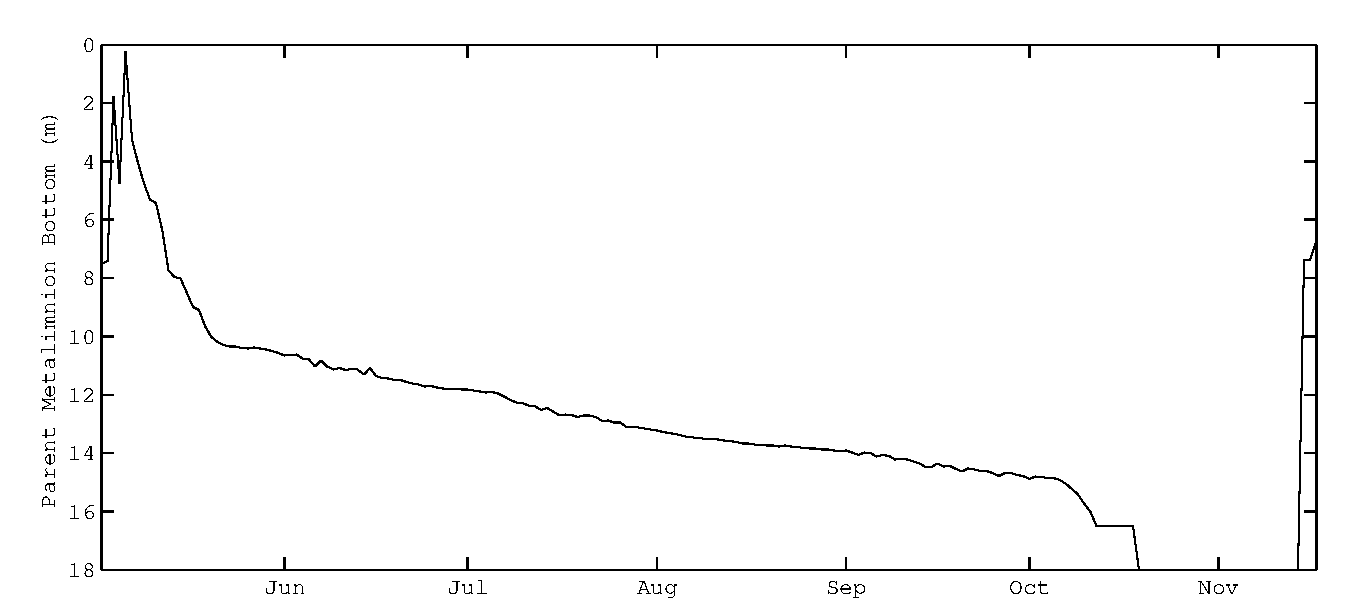
\includegraphics[width=\linewidth]{figures/Sparkling_SmetaB.pdf}
		\end{subfigure}
		\begin{subfigure}{\lafigsize}
			\caption{\label{fig:la:out:N2}Buoyancy Frequency}
			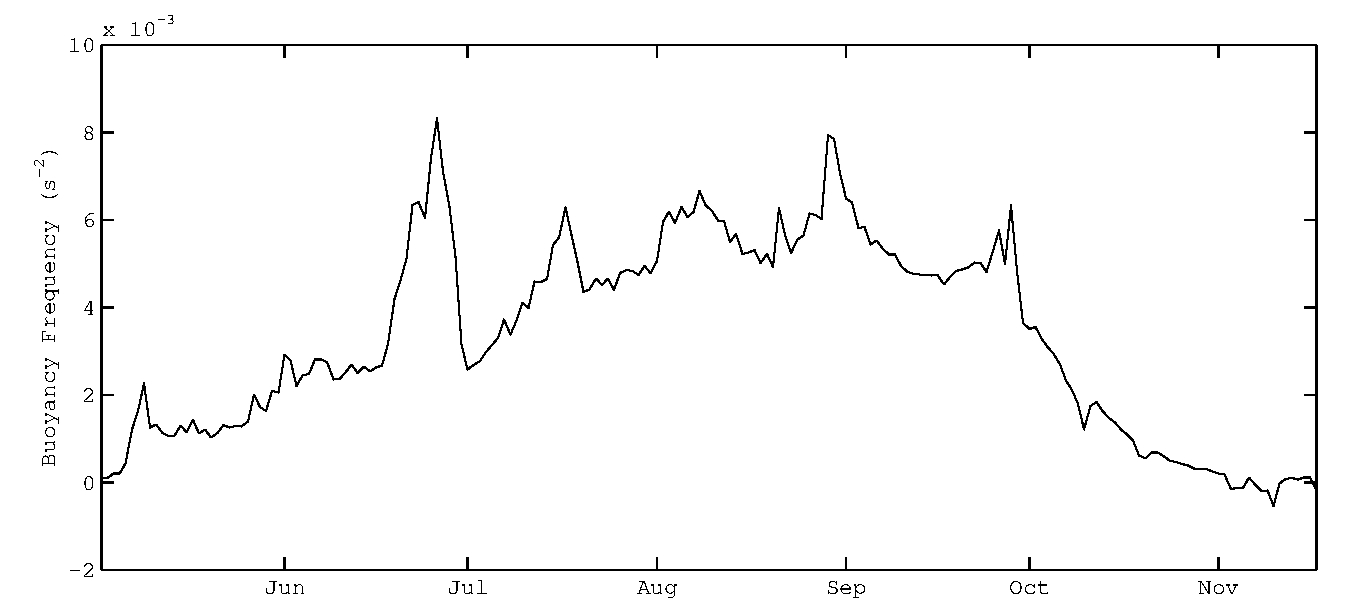
\includegraphics[width=\linewidth]{figures/Sparkling_N2.pdf}
		\end{subfigure}
		\begin{subfigure}{\lafigsize}
			\caption{\label{fig:la:out:SN2}Seasonal Buoyancy Frequency}
			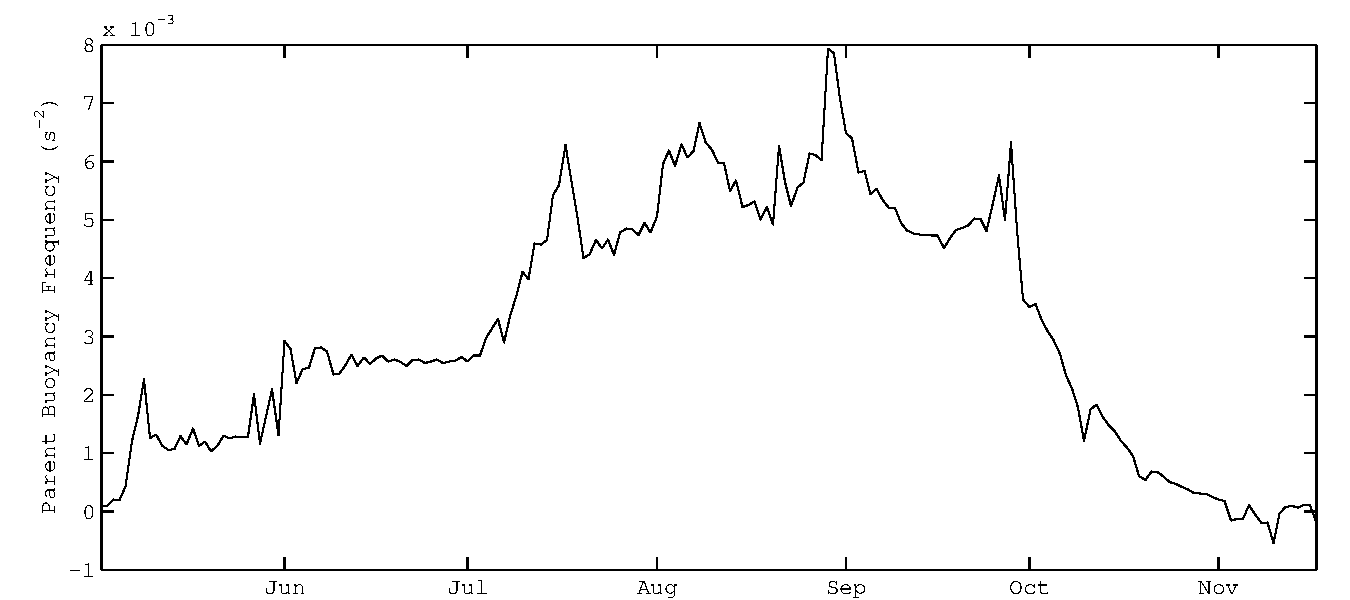
\includegraphics[width=\linewidth]{figures/Sparkling_SN2.pdf}
		\end{subfigure}
		\begin{subfigure}{\lafigsize}
			\caption{\label{fig:la:out:T1}Mode-1 Vertical Seiche Period}
			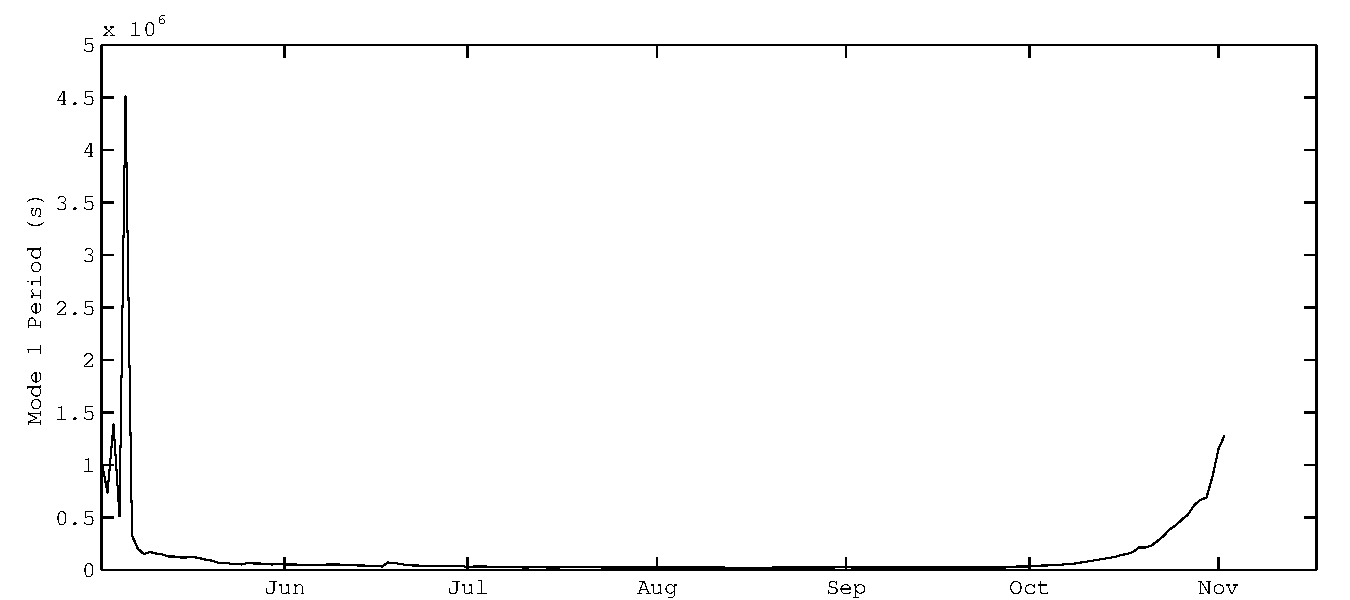
\includegraphics[width=\linewidth]{figures/Sparkling_T1.pdf}
		\end{subfigure}
		\begin{subfigure}{\lafigsize}
			\caption{\label{fig:la:out:ST1}Seasonal Mode-1 Vertical Seiche Period}
			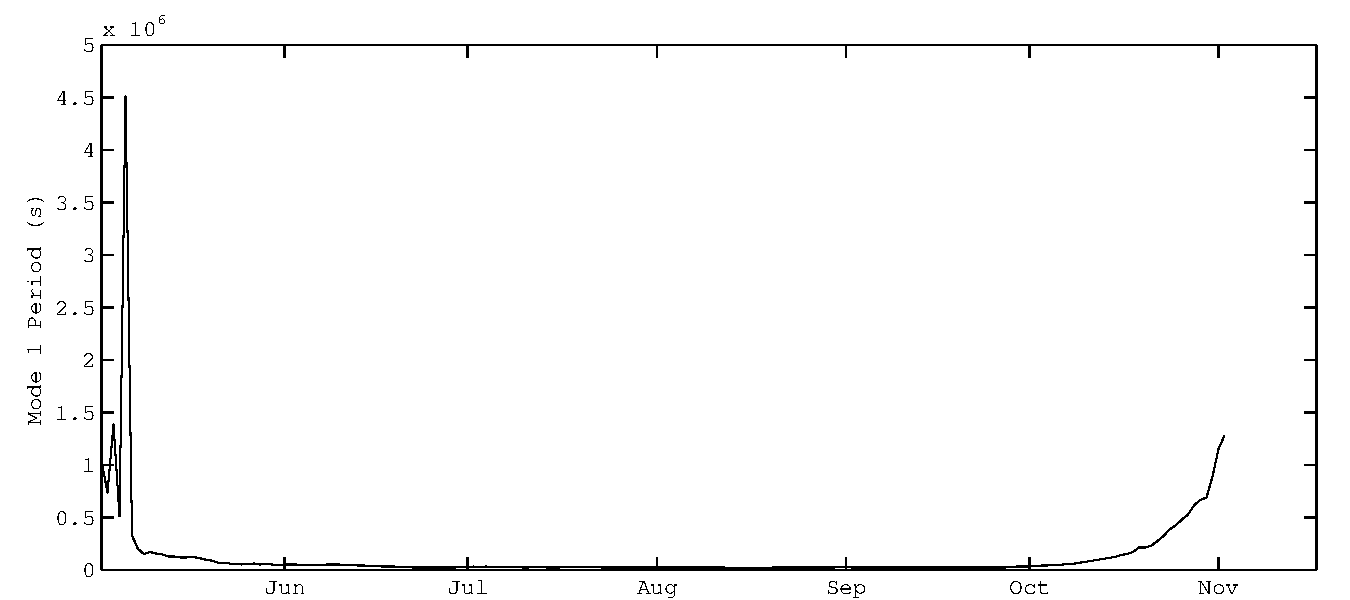
\includegraphics[width=\linewidth]{figures/Sparkling_ST1.pdf}
		\end{subfigure}
		\caption{\label{fig:la:outputs:1}Visualization of \la outputs \emph{(continued on \cpageref{fig:la:outputs:2})}.}
	\end{figure}
	\begin{figure}
		\ContinuedFloat\centering\captionsetup{list=no}
		\begin{subfigure}{\lafigsize}
			\caption{\label{fig:la:out:W}Wedderburn Number}
			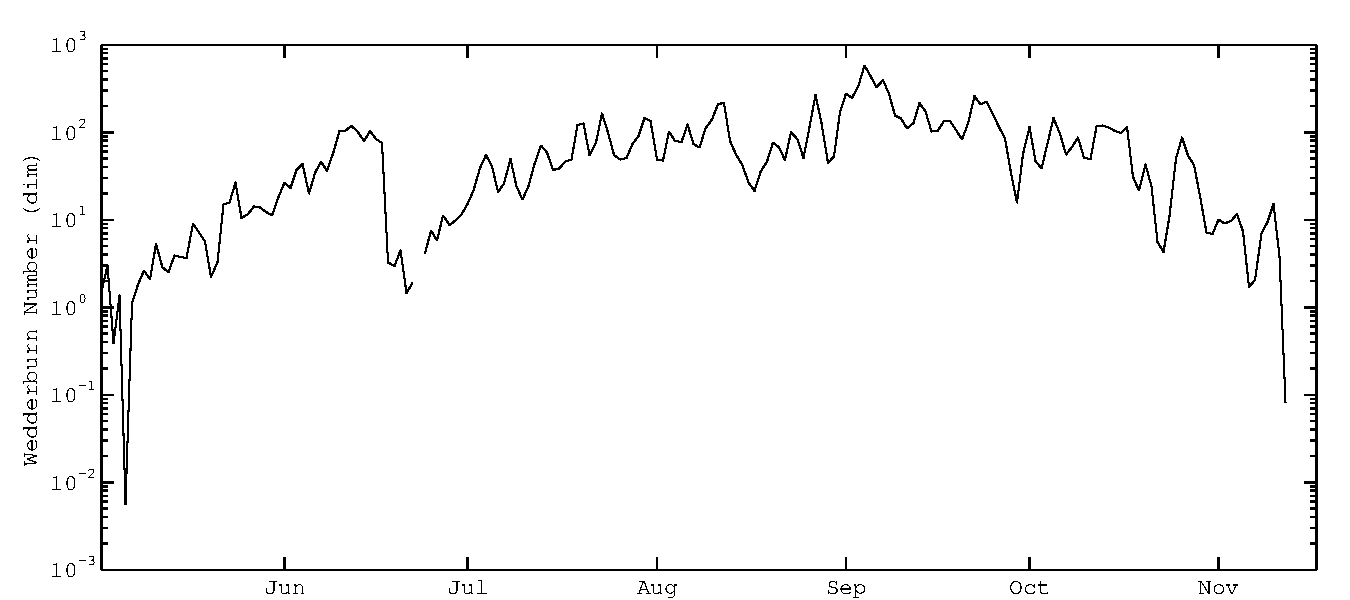
\includegraphics[width=\linewidth]{figures/Sparkling_W.pdf}
		\end{subfigure}
		\begin{subfigure}{\lafigsize}
			\caption{\label{fig:la:out:SW}Seasonal Wedderburn Number}
			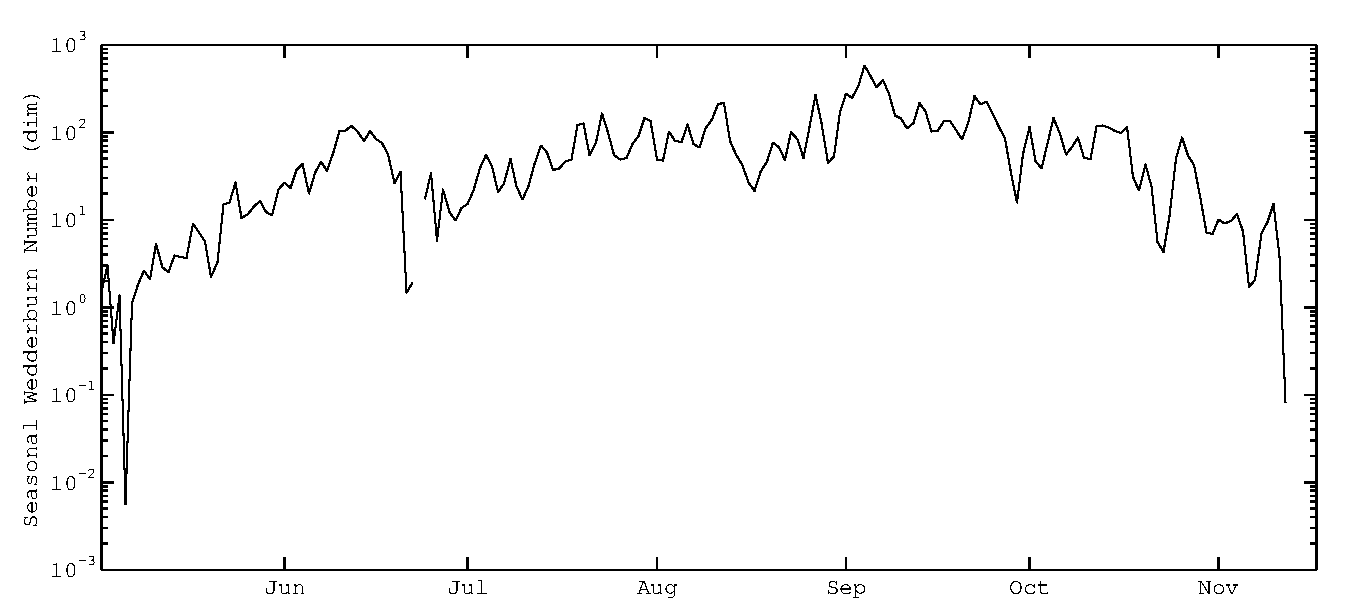
\includegraphics[width=\linewidth]{figures/Sparkling_SW.pdf}
		\end{subfigure}
		\begin{subfigure}{\lafigsize}
			\caption{\label{fig:la:out:thermD}Thermocline Depth}
			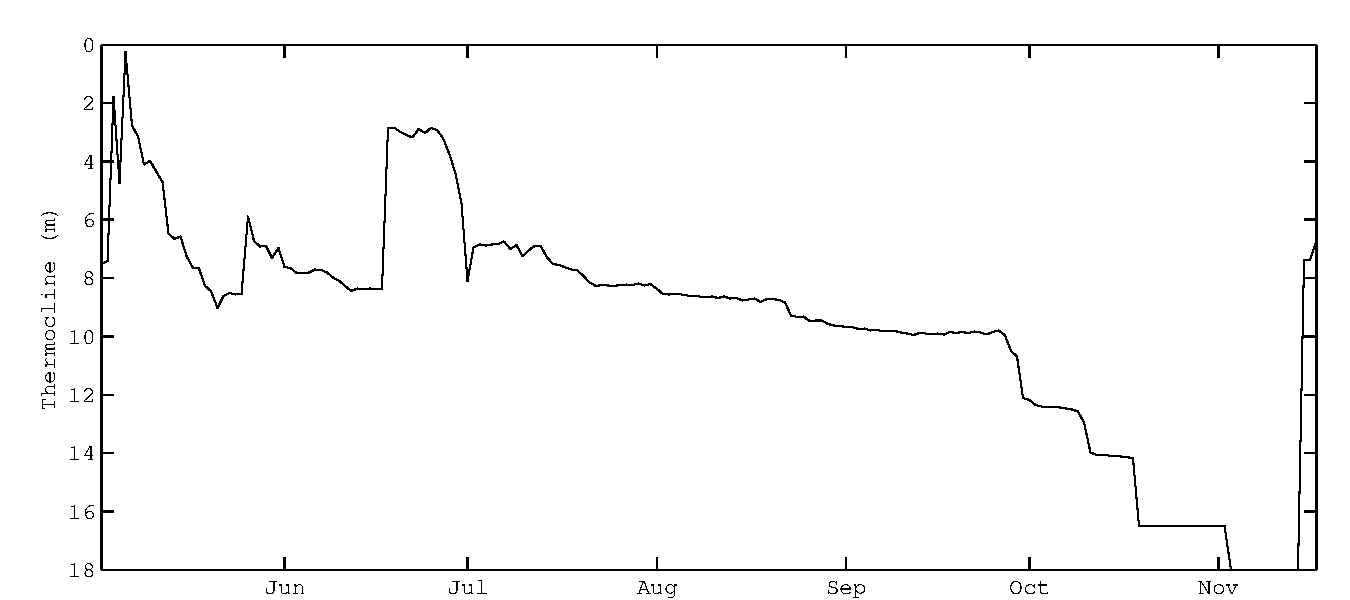
\includegraphics[width=\linewidth]{figures/Sparkling_thermD.pdf}
		\end{subfigure}
		\begin{subfigure}{\lafigsize}
			\caption{\label{fig:la:out:SthermD}Seasonal Thermocline Depth}
			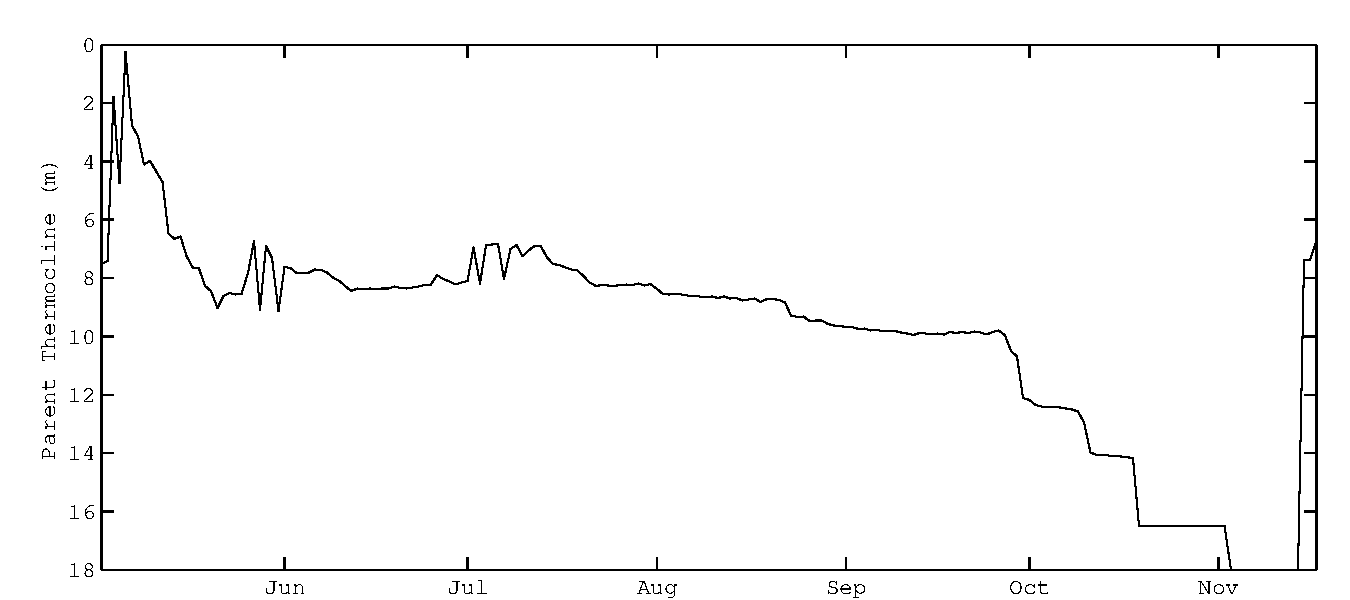
\includegraphics[width=\linewidth]{figures/Sparkling_SthermD.pdf}
		\end{subfigure}
		\begin{subfigure}{\lafigsize}
			\caption{\label{fig:la:out:uSt}$u^{*}$}
			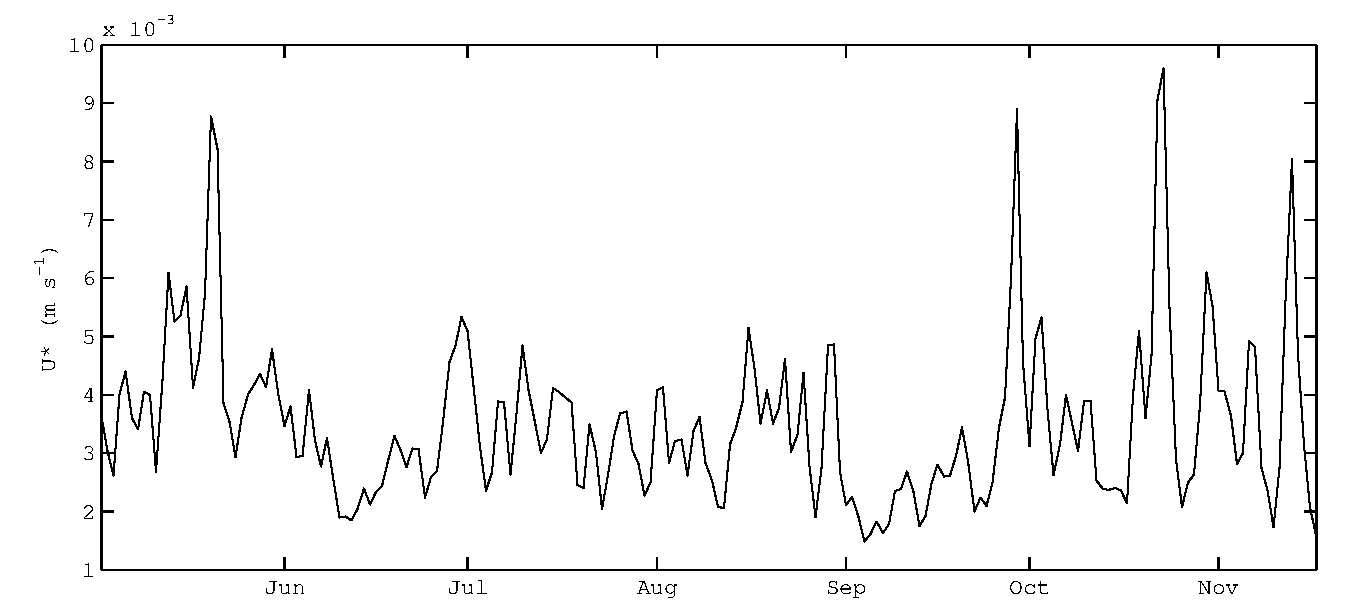
\includegraphics[width=\linewidth]{figures/Sparkling_uSt.pdf}
		\end{subfigure}
		\begin{subfigure}{\lafigsize}
			\caption{\label{fig:la:out:SuSt}Seasonal $u^{*}$}
			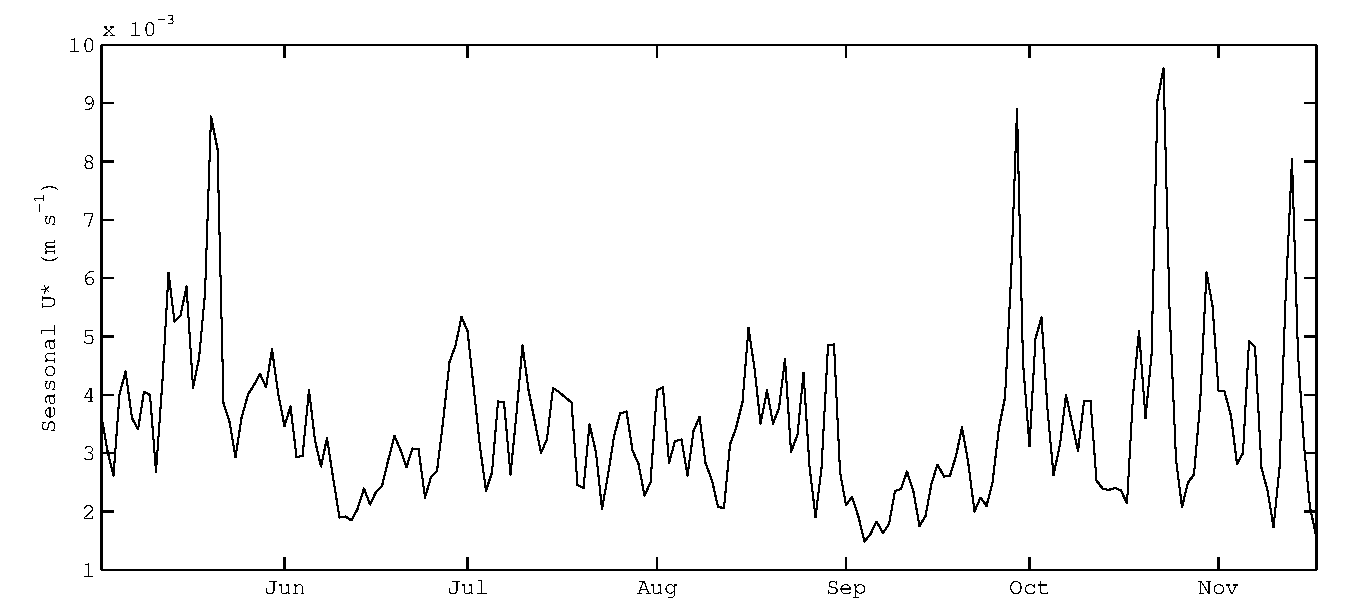
\includegraphics[width=\linewidth]{figures/Sparkling_SuSt.pdf}
		\end{subfigure}
		\begin{subfigure}{\lafigsize}
			\caption{\label{fig:la:out:St}Schmidt Stability}
			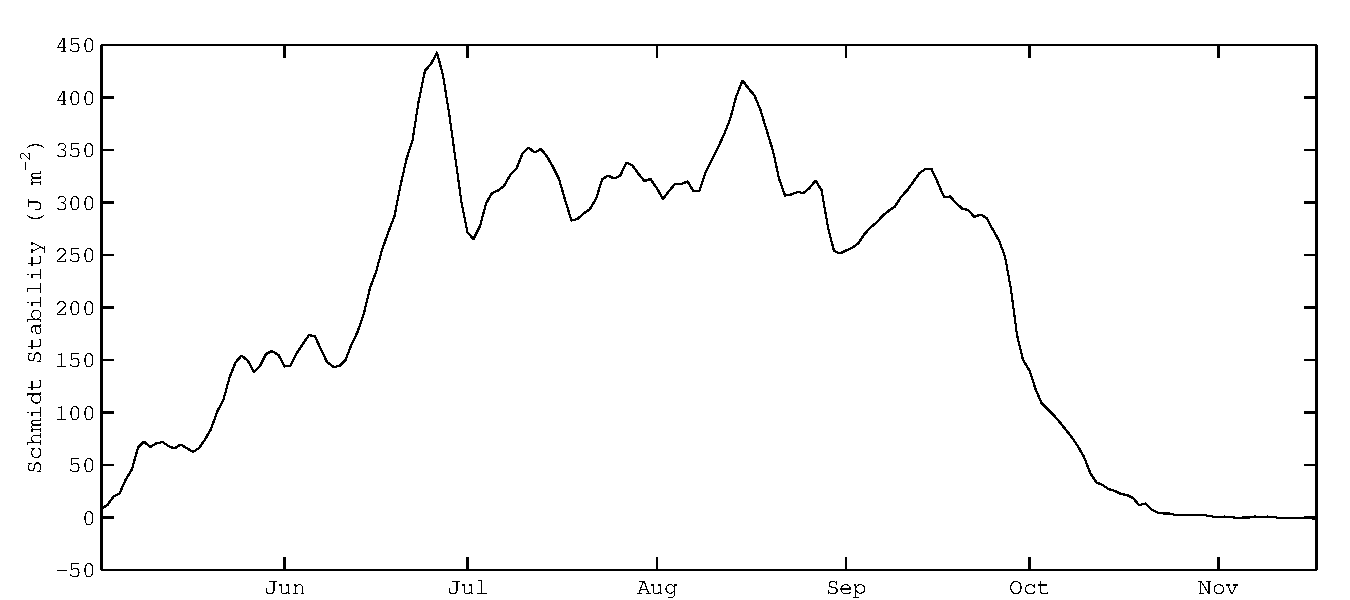
\includegraphics[width=\linewidth]{figures/Sparkling_St.pdf}
		\end{subfigure}
		\begin{subfigure}{\lafigsize}
			\caption{\label{fig:la:out:wndSpd}Wind Speed}
			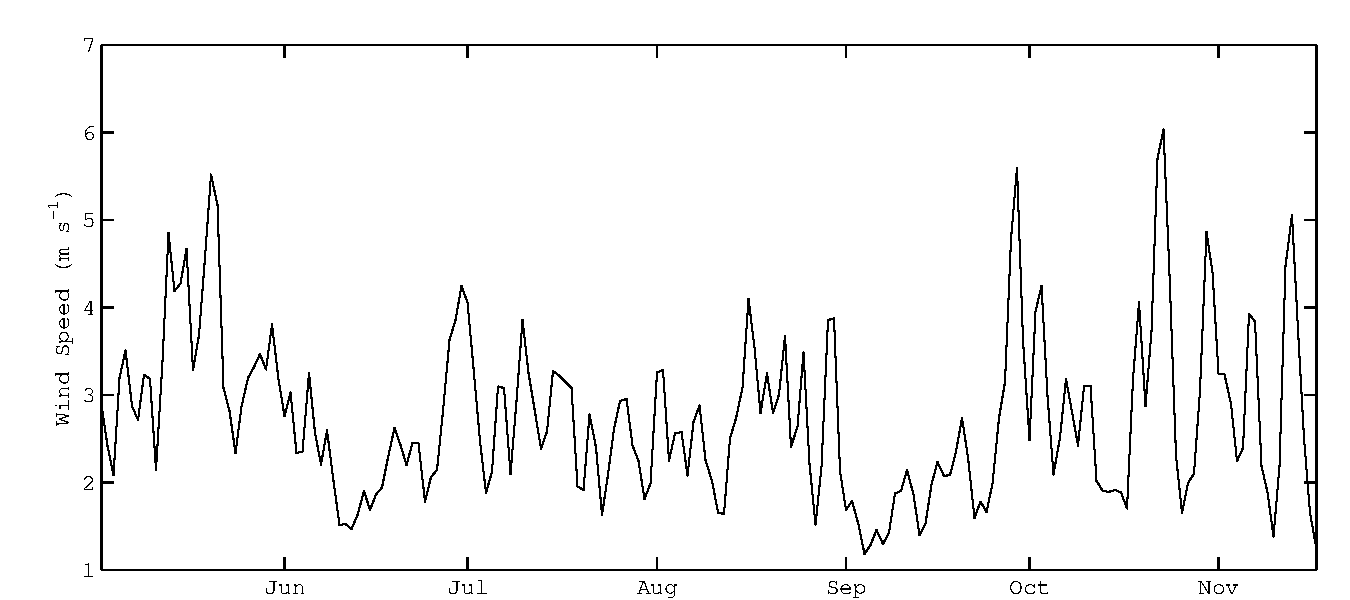
\includegraphics[width=\linewidth]{figures/Sparkling_wndSpd.pdf}
		\end{subfigure}
		\begin{subfigure}{\lafigsize}
			\caption{\label{fig:la:out:wTemp}Water Temperature}
			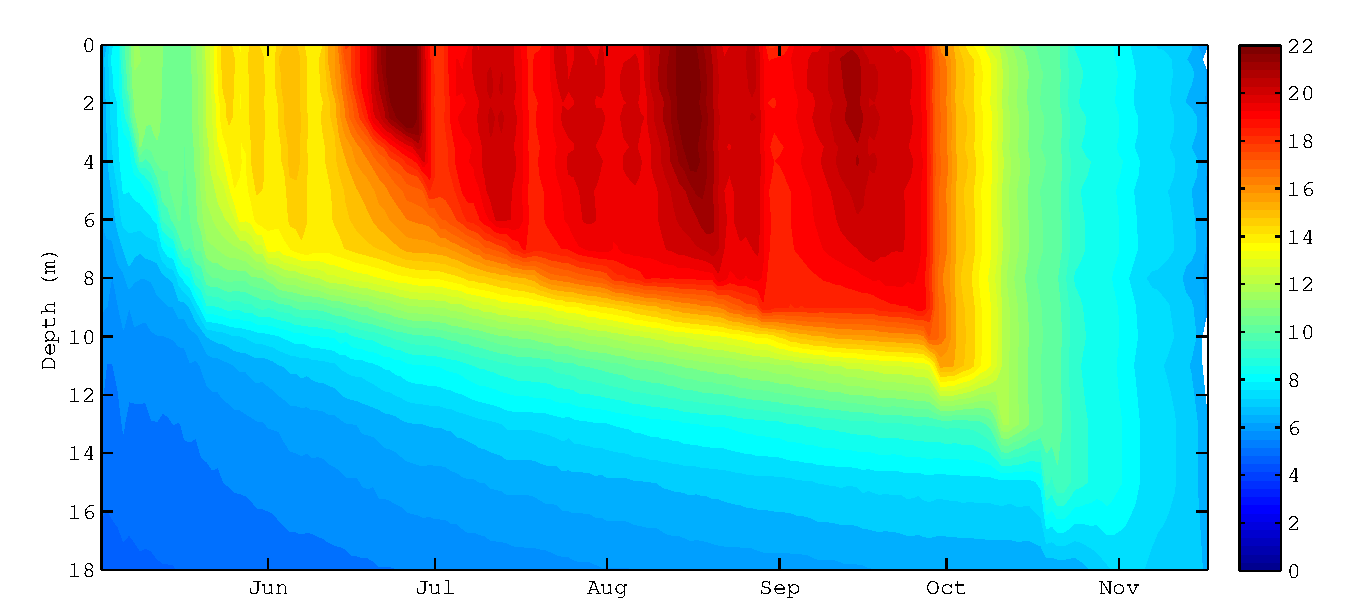
\includegraphics[width=\linewidth]{figures/Sparkling_wTemp.pdf}
		\end{subfigure}
		\caption{\label{fig:la:outputs:2}Visualization of \la outputs.}
	\end{figure}

\chapter{Web Processing Service}
	\label{sec:wps}
	The \ac{WPS} \citep{ogc:wps} is the quasi standard for web based processing of spatiotemporal data \citep{foerster2012live}. It is an open service standard specified by the \ac{OGC} and is embedded in the \ac{OWS} \citep{ogc:ows} environment. Even though the \ac{WPS} is mostly used in the geospatial domain, it's interface is not restricted to spatiotemporal data and also can be deployed in other professional contexts. Within the WPS, it is possible to publish and execute models, algorithms or generic calculations and computations in a standardized web service interface, so called processes. The \ac{WPS} describes a generic interface, that imposes no restrictions on the type of process, their inputs and outputs and so it can encapsulate any kind of algorithm or model. By this, an interoperability is offered, which leads to a number of significant advantages. It adds a layer that hides complexity and permits -- by it's consistency across implementations -- a high level of reusability, flexibility and scalability. Server and client software implementations become reusable and generic client implementations are possible. Scalable and complex computations, like grid \citep[e.g.][]{grid1,grid2,grid3} or cloud computing \citep[e.g.][]{cloud}, as well as super computer processing are hidden behind a simple to use service interface and become accessible.

	The \ac{WPS} specifies mechanisms to discover algorithms and models by offering generic encoding formats for process descriptions and a uniform interface to explore and retrieve these. Besides that, it defines a universal process execution model, that includes request and response encodings, synchronous and asynchronous process executions, long running processes as well as a data encoding for input and output parameters. The interface offers the possibility to retrieve a process output either in a raw format, embedded in a response, or stored in the \ac{WPS} for later retrieval. This facilitates process chaining and enables the subsequent retrieval of process results. The specification describes three different bindings to access a \ac{WPS} using the \acrocitep{HTTP}{ietf:rfc2616}. It may be addressed using \ac{KVP} encoding with HTTP GET, XML encoding with HTTP POST, or clients may use SOAP \citep{w3c:soap1} to access the web service.

	Functionalities are exposed by means of three distinct methods. As every \ac{OGC} web service the \ac{WPS} has a \emph{GetCapabilities} method, that can be used to request a detailed description of the service and its capabilities. It offers a service identification structure which contain information about the organization operating the \ac{WPS}. Also present is a service provider section that contains informational meta data about the service instance which can be used for service discovery. Besides that, detailed information about supported operations, bindings, languages as well as a list of available processes are incorporated.

	The detailed description of a single process may be requested by using the \emph{DescribeProcess} operation. Its response contains informational meta data (like textual descriptions) and the process capabilities in regards to asynchronous execution and response/output storage. Comprehensive information about required and supported inputs, their cardinalities, supported formats and restrictions, and available outputs as well as their supported formats are also included.

	Processes are executed using the \emph{Execute} operation. Besides the necessary input parameters and information about their encoding, the request describes selected outputs that should be generated by the process. Furthermore, it informs the \ac{WPS} whether the process should be executed synchronously or asynchronously and how the results of the process should be encoded.

	\begin{figure}[!htb]
		\centering
		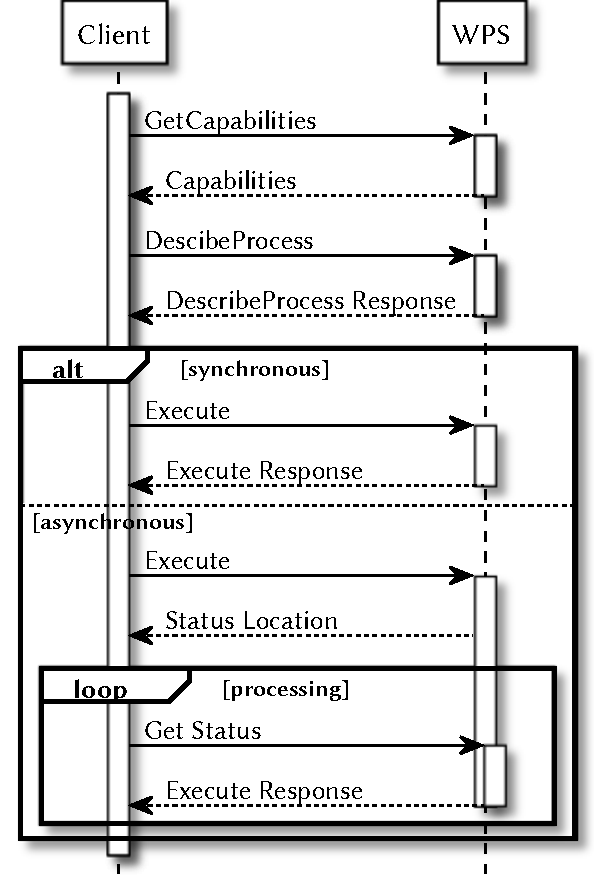
\includegraphics[width=0.40140845070422537\linewidth]{figures/sequence-diagramm-wps.pdf}
		\caption{\label{fig:sd:wps}Typical interaction patterns of the \acl{WPS}: process discovery using \emph{GetCapabilities} and \emph{DescribeProcess} and synchronous as well as asynchronous process execution using \emph{Execute}.}
	\end{figure}

	Typical interaction patterns of the \acl{WPS} are depicted in \cref{fig:sd:wps}. During process discovery, \emph{GetCapabilities} and \emph{DescribeProcess} are used to request a list of available processes and their descriptions. Process execution takes place either synchronously or asynchronously by issuing an \emph{Execute} request to a specific process. In the case of asynchronously process executions, the \ac{WPS} returns an URL to an \emph{ExecuteResponse} which is continuously updated and which the client can request periodically to get the current process status.

	The \ac{WPS} describes three basic types of input and output parameters: \emph{literal}, \emph{complex} and \emph{bounding box} parameters. Complex data parameters are data structures that can be described by a mime type, an encoding and a schema. They can represent raster data, XML structures such as \ac{GML} \citep{ogc:gml} feature collections, \ac{CSV} or any other type of data. This data can be supplied embedded in XML or as a reference to an external HTTP resource. Referenced complex data structures may be requested by using HTTP GET or POST and can transport HTTP headers and any body payload (or reference to one). By this, chaining of \ac{WPS} processes can easily be implemented, either by referencing a previous generated output or even by encoding another \emph{Execute} call into the reference. Literal data can be represented by a single string value. The value is described by a data type and can be accompanied by a unit of measurement. Typical data types include single strings, URIs, boolean values, dates and integral or decimal numbers. Bounding box data represents a rectangular region of arbitrary dimension which is described by a \ac{CRS}.

	As shown in this chapter, there are several benefits that can be expected by using the WPS. Especially in the context of domain specific models, the interoperability and reusability can be increased significantly. Until now, the \la can not be deployed in a web based processing chain and has to be executed in a manual procedure. Web based execution is currently realized by using a web form that allows remote execution of the \la. This way of proceeding presupposes the recourse to specialized software or scripts for automation and can be characterized as very disadvantageous, e.g. for the reuse of the developed model in other projects. The following section focuses on a WPS that allows the deployment of models developed in MATLAB -- like the \la -- as WPS processes with the purpose of profiting from the positive aspects of standardized web based processing solutions.

\chapter{MATLAB WPS}
	MATLAB\fu{http://www.mathworks.com/products/matlab/} is a closed source, commercial software by The MathWorks, Inc. for numerical computation, visualization and programming. It features a high-level programming language as well as an cross-platform (Windows, Linux and Mac OS X) interactive desktop environment. Initially developed for matrix computations (hence \emph{MAT}rix \emph{LAB}oratory)\fu{http://www.mathworks.com/company/newsletters/articles/the-origins-of-matlab.html}, today MATLAB is widespread across different domains in academics, engineering and industry. The base program is extensible by using so called \emph{toolboxes}, that add functionalities for various domains, like statistics, curve fitting, neural networks, image processing, economics, bioinformatics or signal processing. Besides that, functions, algorithms, files or toolboxes can be installed through \emph{MATLAB Central}, a repository of user contributions. These are mostly licensed under the two-clause BSD license\fu{http://opensource.org/licenses/bsd-license.php}\fu{http://www.mathworks.com/matlabcentral/FX_transition_faq.html}.

	Creating a specific \ac{WPS} process implementation for the \la would be possible. Considering the wide spread usage of MATLAB based scripts and applications, a generic solution, that enables the easy deployment of MATLAB based functionalities as \ac{WPS} processes would have a huge benefit for the geospatial community as well as for the the acceptance of the \ac{WPS} across disciplines. A generic \emph{MATLAB WPS} would not only open the \la for an interoperable usage in existing web processing chains, but would also make existing models and algorithms implemented in MATLAB instantly available to a larger audience and can increase reusability of software components and exchange between different areas of research, development and business. Considering the diversified fields MATLAB is used in, a software component such as a MATLAB WPS can not assume an extensive programming experience beyond MATLAB. Domain experts developing models or algorithms in MATLAB should be able to offer a MATLAB script or function as a \ac{WPS} process using a simple and straightforward procedure, without any knowledge of other programming languages or a comprehensive expertise in web services or their development. To accomplish this, switch from MATLAB to other languages should not be required, and rather complex and verbose process descriptions should not be manually be written, but automatically generated. A key goal of the MATLAB WPS is to expose existing models and algorithms as \ac{WPS} processes. Therefore, the procedure to convert a MATLAB script or function should not require intrusive changes to be compatible with the MATLAB WPS.

	Approaches to offer data analysis and modeling languages like MATLAB as \ac{WPS} processes do already exist. Specially emphasized should be the \emph{WPS4R} \citep{wps4r} project that creates WPS processes from scripts written for the statistical analysis environment \emph{R} \citep{gnur}. Written as a module for the \ftn \ac{WPS} implementation, it shares many requirements and challenges with a MATLAB WPS. R is also an environment used mostly by domain experts and features a massive amount of existing models and algorithm implementations. These are worth to be opened to the web processing environment and to be made available to a broader user base using interoperable standards like the \ac{OGC} \acl{WPS}.

	\lstinputlisting[label={lst:r:annotation},
					 caption={Example for a comment containing annotations used by WPS4R \citep{wps4r}.},
					 language=R]{listings/wps4r-annotations.r}

	WPS4R takes an R script and executes it on a remote or local R instance using \emph{Rserve} \citep{rserve}. In contrast to the \ac{WPS} interface which explicitly states types of input and output parameters to allow service discovery and the usage of generic clients, R is a weakly and dynamically typed language. By this, the \ac{WPS} is not able to parse the script and determine appropriate input and output parameter types, as these are only available at runtime. To bind static types to input and output parameters, an annotation mechanism was developed which is also capable to detail input/output and process meta data. In contrast to other programming languages, like Java \citep{jsr175} or C\# \citep{ecma335}, R does not feature a native annotation mechanism. Because of this, the annotations are encoded as comments featuring special keywords (\emph{wps.in}, \emph{wps.out} and \emph{wps.des}), followed by a key value list representing the necessary information to generate a process description (see \cref{lst:r:annotation}). During process execution, WPS4R will populate the described input parameter variables using \ac{WPS} inputs, execute the script, read the specified output variables from the R session and transform them to WPS outputs. The usage of annotations embedded in comments support the deployment of R functionalities as WPS processes by providing a single script file that the WPS4R can parse.

	Literal input parameters are translated into native R types, whereas complex inputs are transferred as files to a temporary working directory. Complex input and output parameters have to be described by a single keyword, denoting the mime type of the parameter, that has to be registered to WPS4R using a configuration file. Describing complex inputs and outputs using \emph{schema} or \emph{encoding}, or using about any mime type without changing the WPS4R configuration, is not possible. This may be caused by the reduced expressiveness through the usage of a structureless description format (e.g. denoting multiple supported complex input formats, would be hard to specify). Scripts are run on globally configured Rserve connections. Different remotes for different processes or a load balancing between multiple remote nodes running R are not possible. Furthermore, the easy deployment of scripts consisting of multiple files is currently not possible.

	The comment based approach taken by WPS4R has several advantages like having \ac{WPS} configuration and actual code side by side (which results in less maintenance effort), but also introduces considerable drawbacks, especially if the annotation mechanism should be applied to MATLAB. Conveying important information in comments can be problematic. Even though there are many examples where comments are used (e.g. to generate documentation as seen on the example of Javadoc \citep{javadoc}) these are often standardized at language level or include a large user base and a wide support in editors and development environments. The syntax of a custom comment based annotation mechanism as used in this approach, can not be verified in editors or interpreters. By this and the unstructured notation of comments, the approach becomes heavily prone to user error, that can not be detected before the deployment to a WPS instance. Additionally, annotations are not actually bound to any language construct, but just happen to be in the same file.

	Typical MATLAB programs would not benefit from combining annotations and scripts in a single file, as it is common practice -- or even a requirement to access a function from outside -- to place a function in its own file. By this, MATLAB programs tend to consist of multiple files, and can not easily deployed as single script files.

	\dots

	In contrast to R, MATLAB offers multiple return values of functions as a native language feature (see \cref{lst:matlab:example:fun}). Through this, MATLAB functions are able to directly represent a \ac{WPS} process, and the MATLAB WPS should use MATLAB functions instead of scripts to offer functionalities as WPS processes. As stated before, MATLAB is a weakly and dynamically typed language, and the parsing of a function signature can not create a statically typed binding as the \ac{WPS} standard requires. For this, an additional description mechanism has to be developed that allows the semi-automatically generation of process descriptions. This should be done without extensive knowledge of web service development or programming languages. Also the deployment of existing MATLAB functions should be a straightforward non-intrusive process. Similar to R, MATLAB instances are single threaded, and so can only process one WPS process execution a time. Moreover, and contrary to R, opening the MATLAB workbench even in a headless mode (i.e. without any user interface) can take considerable time. This requires an efficient usage of MATLAB instances, especially the reuse of already started MATLAB instances to reduce latency of process executions. Complex inputs should be usable inside of MATLAB without restrictions to any format, and without the need to change any configuration files.

	\lstinputlisting[label={lst:matlab:example:fun},
				 	 caption={MATLAB example function that calculates statistical characteristics (mean and standard deviation) of an input vector.},
					 language=Matlab]{listings/matlab-stat-function.m}

	This chapter will outline the conceptualization and implementation of a MATLAB WPS by describing its architecture and configuration mechanism. Furthermore, details of the conversion between MATLAB and WPS types will be discussed and legal implications of offering commercial software as web services will be shortly examined. Finally, the generic capabilities of the MATLAB WPS will be used in order to offer the \la as a WPS process.

	\section{Architecture}
		The MATLAB WPS features a multi-tier architecture to offer MATLAB functions as \acl{WPS} processes. A detailed sequence diagram depicting a MATLAB WPS process execution can be seen in \cref{fig:sd:mwps}. An incoming WPS \emph{Execute} request is accepted by the MATLAB WPS (\hyperref[fig:sd:mwps]{step~1}). The \emph{Execute} request is verified (e.g. no missing inputs, inputs within the range described by the process description, etc.) and then translated into a MATLAB request (\hyperref[fig:sd:mwps]{step~2}). This request is send via a WebSocket connection to a configured MATLAB server (\hyperref[fig:sd:mwps]{step~3}). The MATLAB server maintains a pool of MATLAB instances and will dispatch the request to one of these as soon as one becomes available (\hyperref[fig:sd:mwps]{step~4}). The instance transforms the MATLAB request into MATLAB syntax (\hyperref[fig:sd:mwps]{step~5}) and evaluates the MATLAB command in an associated MATLAB session. After this (\hyperref[fig:sd:mwps]{step~6}), the return values are read from the session (\hyperref[fig:sd:mwps]{step~7}) and encoded as a MATLAB response (\hyperref[fig:sd:mwps]{step~8}). It is then passed through the MATLAB server (\hyperref[fig:sd:mwps]{step~9}) to the MATLAB WPS (\hyperref[fig:sd:mwps]{step~10}). The MATLAB WPS process translates the MATLAB response to a WPS \emph{Execute} response (\hyperref[fig:sd:mwps]{step~11}) and returns it to the client (\hyperref[fig:sd:mwps]{step~12}).

		\begin{figure}[!htb]
			\centering
			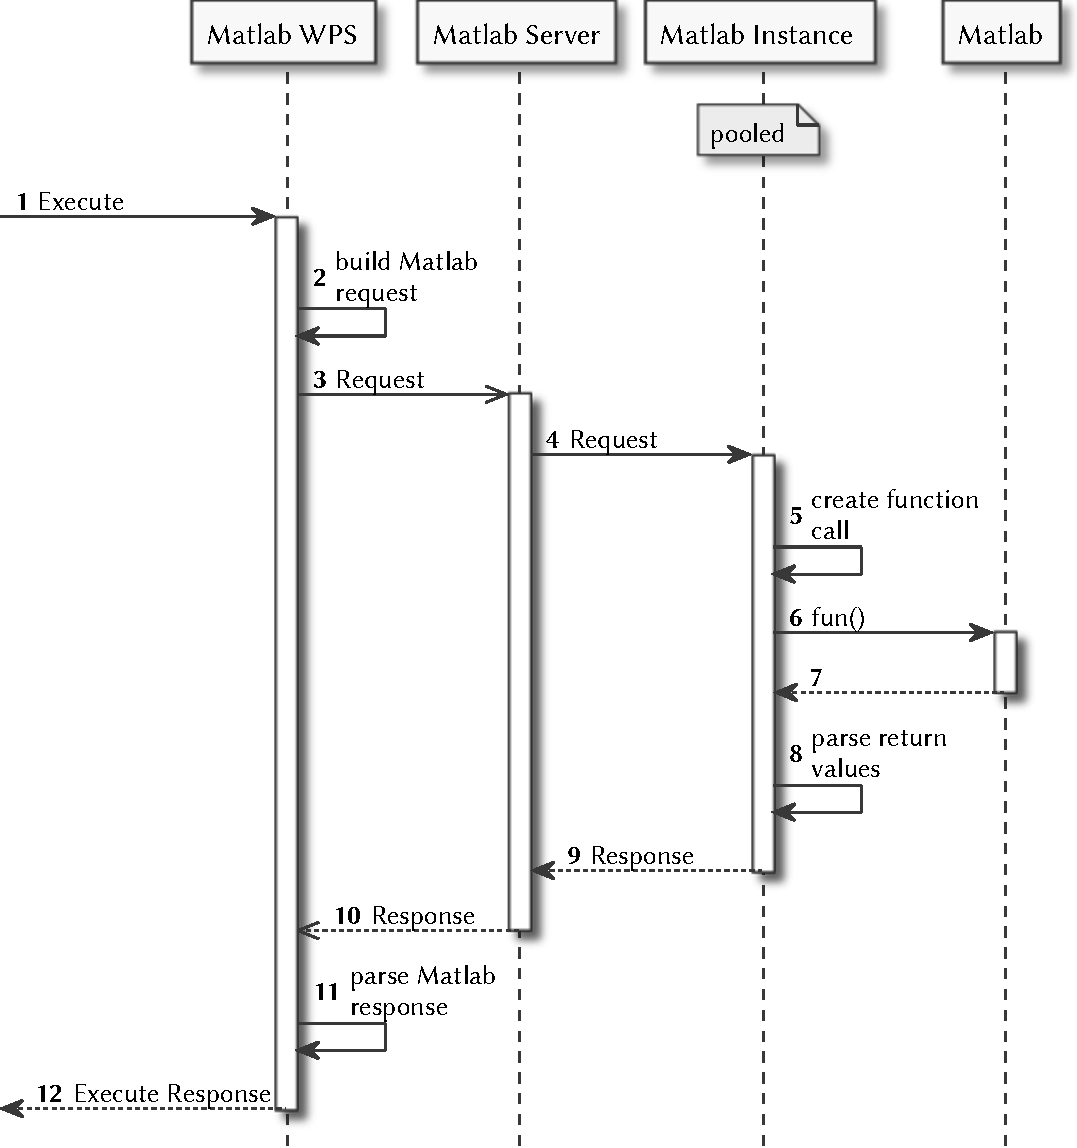
\includegraphics[width=0.6788732394366197\linewidth]{figures/sequence-diagramm-mwps.pdf}
			\caption{\label{fig:sd:mwps}Sequence diagram of a MATLAB WPS process execution.}
		\end{figure}

		Besides an option to run the MATLAB server locally, all communication between the MATLAB WPS and MATLAB server is done over WebSockets \citep{ietf:rfc6455}. WebSockets are defining a TCP-based protocol that creates a bidirectional communication channel between client and server. A primary goal of WebSockets is to bring the benefits of efficient full-duplex communication to the web browser environment. This is accomplished by an HTTP compatible socket initiation mechanism (see \cref{lst:websocket}). A client opens a new WebSocket by issuing an HTTP request to the server, in which it requires an upgrade to the WebSocket protocol. Afterwards, the connection is kept open and both client and server can send messages to the opposing party. These messages are transported using one or more text or binary frames and allow an efficient bidirectional information exchange. By using HTTP for the initial handshake, WebSockets can be used in most proxy setups and despite the presence of firewalls that filter non HTTP traffic and can facilitate HTTP's access control mechanisms and client side security measures like \acl{CORS} \citep[\acs{CORS},][]{w3c:cors}.

		\lstinputlisting[caption={WebSocket opening handshake using a HTTP upgrade request \citep{ietf:rfc6455}.},label={lst:websocket}]{listings/websocket-handshake.txt}

		Even though the opening handshake is using HTTP, WebSockets do not conform to the HTTP protocol. To ensure that a web server can handle WebSocket connections, the client sends the header \emph{Sec-WebSocket-Key} in the opening request, containing 16 bytes of random data in base 64 encoding \citep{ietf:rfc4648}. The server has to append the Globally Unique Identifier \cite[GUID,][]{ietf:rfc4122} \emph{258EAFA5-E914-47DA-95CA-C5AB0DC85B11} to the header value and return the base 64 encoded SHA-1 \citep{NistFIPS1803} hash sum using the \emph{Sec-WebSocket-Accept} header field. Because of the incompatibility with the HTTP protocol, WebSockets define two separate URL schemes: \emph{ws} for normal WebSocket connections and \emph{wss} for secure WebSocket connection, which resemble the HTTP and HTTPS protocol and share their default ports 80 and 443.

		The WebSocket protocol is accompanied with an HTML5 JavaScript \ac{API} \citep{w3c:ws} that is implemented in all recent versions of major desktop browsers\footnote{And with the exception of Opera Mini also mobile browsers.} \citep{caniuse}. Besides that, WebSocket client and server implementations for nearly all programming languages (e.g. R\fu{https://github.com/rstudio/R-Websockets}, C\fu{http://libwebsockets.org/trac/libwebsockets}, C\#\fu{http://msdn.microsoft.com/library/system.net.websockets.websocket.aspx}, Java\fu{https://jcp.org/en/jsr/detail?id=356}) exist.

		As previously noted, function calls are used as the central element of MATLAB WPS processes. Using the native language feature of multiple return values, WPS processes can be represented as MATLAB functions one to one. The MATLAB WPS is not designed to easily interface MATLAB with the WPS implementation to allow process development from within the WPS, but to allow the deployment of any MATLAB model using a WPS. Because of this, the MATLAB WPS only offers functionalities to evaluate a single function call and is not required to evaluate scripts, parse MATLAB code or maintain variable references. By this, a very thin implementation is possible and the configuration and maintenance efforts are reduced to a minimum.

		The components \emph{MATLAB server} and \emph{MATLAB instance} as shown in \cref{fig:sd:mwps} are developed separately from the MATLAB WPS and can be easily used in other contexts. This \emph{matlab-connector} consists of a small Java CLI application (the server) and an associated Java client library used in the MATLAB WPS, that offers a simple \ac{API} to build MATLAB requests. The server component is started on the machine on which MATLAB is installed, and then offers a configurable amount of headless MATLAB instances using a small WebSocket server. The MATLAB instance communicates with a \ac{JVM} exposed by the MATLAB program using a Java \ac{RMI} wrapper called \emph{matlabcontrol}\fu{https://code.google.com/p/matlabcontrol/}. As previously noted, MATLAB instances are, even in headless mode, heavy weight applications that require a considerable amount of resources and time to start. MATLAB instances are created at server startup and then are used to process requests. By reusing and preallocating a fixed amount of instances, the pooling of MATLAB instances reduces latency for WPS processes and saves resources on the server machine.

	\section{Configuration}
		\label{sec:matlab:conf}
		Because of the aforementioned problems regarding comment annotations, the MATLAB WPS features another configuration mechanism. Process configurations are conveyed using YAML \citep{yaml} which facilitate a particular human-readable syntax. It allows easy structuring of data without delimiters like quotation marks or braces, but allows these e.g. to enable a more compact syntax. The structure of YAML has close resemblance with JSON (which is actually a valid subset of YAML since version 1.2) and features the same basic types of scalars, sequences and associative arrays (maps), but has additional features that make it more expressive. This includes comments, multi-line strings, references, multi-document files, sets, complex key types for maps, ordered/unordered maps and maps that allow duplicate keys.
		\lstinputlisting[language=YAML,
						 label={lst:matlab:example:yaml},
						 caption={MATLAB process configuration describing the function in \cref{lst:matlab:example:fun}.},
						 morekeywords={function,connection,identifier,version,inputs,outputs,type,maxOccurs,title,abstract}]{listings/matlab-stat-process-configuration.yaml}
		Configuration files for the MATLAB WPS can contain multiple process configurations expressed as an associative array. These are describing a MATLAB function, their input and outputs as well as where the function should be executed. It resembles the basic structure of a WPS process description while concealing the verbosity and complexity of XML. \cref{lst:matlab:example:yaml} shows an example process configuration for the function displayed in \cref{lst:matlab:example:fun}. The process description generated from the YAML configuration can be found in \cref{lst:matlab:example:desc}.

		\lstinputlisting[label={lst:matlab:example:desc},
						 caption={[Process description generated from the configuration in \cref{lst:matlab:example:yaml}.]Process description generated from the configuration in \cref{lst:matlab:example:yaml} (see \cref{sec:xmlnamespaces} for omitted XML namespaces).},
						 language=XML]{listings/matlab-stat-process-description.xml}
	 	Top level attributes are describing the process itself, whereas \emph{inputs} holds a sequence of input descriptions and \emph{outputs} a sequence of output descriptions in the very same order the function is defined. The function to describe is denoted by the keyword \emph{function}. \emph{identifier}, \emph{title} and \emph{description} are directly mapped to their equivalent in the \ac{OGC} name space. The attribute \emph{maxOccurs} holds either an integral number or the special value \emph{unbounded} which will be translated to the platform specific maximum possible value (typically the greatest possible integer value). Data types, described under the keyword \emph{type}, are translated to their respective XML data type. Complex data types can be described using a map containing a combination of \emph{mimeType}, \emph{schema} and \emph{encoding}. Bounding box inputs are described using a map containing the keyword \emph{crs}, which holds one or more supported \ac{CRS}.

		The attribute \emph{connection} denotes how the function should be executed. The keyword \emph{local} will cause the MATLAB WPS to start a pool of MATLAB instance in the current working directory. The function has to be either at this path or at any other path searched by MATLAB. Other possible values for \emph{connection} are URIs in the \emph{ws}, \emph{wss} or \emph{file} scheme. The latter will start a connection pool inside the specified directory, while a WebSocket URL will cause the MATLAB WPS to connect to the remote server and will run the function there. In both cases, the file containing the function has to be able to be found in the MATLAB search path.

		Through the very clear and concise YAML notation, complex process description can be easily written in a human readable format, which is way easier to maintain than custom annotations in inline comments. It results in a less error prone procedure for unexperienced domain experts, whereas advanced users are able to benefit from advanced YAML features. Furthermore, future enhancements and additions can be easily implemented backwards compatible.
	\section{Type Mapping}
		\label{sec:matlab:type}
		MATLAB, like any other language, has a wide variety of data types. These include numeric types -- floating point numbers in single (\unit{32}{\bit}) and double (\unit{64}{\bit}) precision and signed and unsigned integers in \unit{8, 16, 32 and 64}{\bit} size -- logical, character/string types as well as structures, tables, cell arrays and function handles. Except for the latter, all of these types have the form of (possible multidimensional) arrays \citep{matlab}.

		As previously described, the \acl{WPS} specification knows three different types of data: literal, complex and bounding box data.
		\ac{WPS} Literal data is mostly converted to their respective native MATLAB data type, but due to limitations in the MATLAB \ac{API}, this is not always possible. The \ac{API} exposed by MATLAB transfers every numerical type as floating point numbers of double precision. By this, an efficient handling of other basic data types like integral numbers or single precision floating point numbers is not possible. Within the WPS specification and implementation, these data types are each handled differently, but due to the limitations exposed by the MATLAB interface, MATLAB processes have to reduce precision on their own in order to reduce memory usage.

		Single and multiple occurrences of input parameters can be handled in MATLAB in the very same way, because every basic data type consists not only of a single value, but an array of it's type. The sole exception are string based data types, which are represented as an array of characters. Placing several strings in an array results in an concatenated string and so a MATLAB \emph{cell} is used for these data types. Boolean values are represented as \emph{logical} 0 or 1 or a respective array and time stamp values are converted to their numerical representation\footnote{A double value containing the fractional number of days since the January 0, 0000.}.

		Bounding box input data is mapped to a \emph{struct} consisting of the fields \emph{crs} and \emph{bbox} holding the \ac{CRS} identifier and a two-dimensional array with the upper and lower corner of the bounding box respectively. This format is also expected for bounding box outputs.

		Complex data is neither parsed nor converted using the MATLAB WPS. It is transferred to a temporary file and passed to the MATLAB function as a file name. For complex outputs, the MATLAB functions saves them to a temporary file and returns the file name. The file is read by the MATLAB WPS and deleted when the process finishes. By delegating the parsing of complex data inputs to the MATLAB function, the WPS is independent from specific data formats -- both in case of specific MATLAB classes and in case of different XML or binary encodings at the WPS end -- and can easily be adopted to existing MATLAB models.

		The usage of complex outputs is currently limited to a single format. Even though the WPS specification allows the request of different formats (e.g. a raster or image can be requested as PNG, JPEG or TIFF, or a feature collection may be requested in different XML schemata), the MATLAB WPS does not offer this feature to MATLAB processes. This is owed to the MATLAB based handling of complex inputs. To become independent of file formats and encodings, the MATLAB WPS can not be used to transform inputs or outputs between different formats. While the inputs and outputs of different format still could be created and consumed on the MATLAB process side, this possibility was neglected to ease MATLAB process development and to allow a more simple transformation of existing MATLAB models.

		MATLAB lacks a value to represent the absence of a value (often denoted as \emph{null}, \emph{nil}, \emph{none} or \emph{nothing} in other programming languages). Even though MATLAB supports optional parameters in function calls, it does not support named function parameters, and a function can only interpret the amount of input parameters to determine if an optional parameter is present or not. As WPS processes can contain a multitude of optional input parameters, the value \emph{NaN} \citep{ieee:754:2008}, which represents an undefined or unrepresentable numeric value and so comes close to a null value, is used to transport absent optional input parameters, regardless of their type.

		The WPS specification offers the possibility to only request specific outputs of a process. This enables the process to only compute the outputs that are really needed and thus can reduce the time needed for process executions. The MATLAB WPS currently does not feature not mechanism and MATLAB functions are required to compute all outputs regardless which are requested by a client.
		%%% move this somewhere else?
		To overcome this issue, the requested output identifiers could be saved in a globally accessible environment variable. In addition to this, other contextual information could be conveyed using this method, e.g. the WPS service URL, which was used to execute the process or other meta data that the function may use.

		\begin{table}[!htb]
			\sffamily
			\centering
			\caption[Mapping between WPS data types and MATLAB types.]{\label{tab:matlab:typemapping}Mapping between WPS data types and MATLAB types. Absent optional parameters are denoted by \emph{NaN} ($1\times1$).}
			\begin{tabular}{@{}llcc@{}}
				\toprule\toprule
				&
				& \multicolumn{2}{b}{Matlab Type}\\
				&
				& \multicolumn{1}{b}{Single}
				& \multicolumn{1}{b@{}}{Multiple}\\
				\midrule
				\multicolumn{2}{@{}l}{\textbf{Complex Data}}
				& char ($1\times{}m$)
				& cell of chars ($1\times{}n$)
				\\
				\midrule
				\multicolumn{2}{@{}l}{\textbf{Bounding Box Data}} & struct ($1\times1$) & cell of structs ($1\times{}n$)\\
				\midrule
				\textbf{Literal Data}
				& xs:string
				& \multirow{2}{*}{char ($1\times{}m$)}
				& \multirow{2}{*}{cell of chars ($1\times{}n$)}\\
				& xs:anyURI\\
				\cmidrule(r){2-4}
				& xs:byte
				& \multirow{7}{*}{double ($1\times1$)}
				& \multirow{7}{*}{double ($1\times{}n$)} \\
				& xs:short\\
				& xs:int\\
				& xs:long\\
				& xs:integer\\
				& xs:double\\
				& xs:float\\
				\cmidrule(r){2-4}
				& xs:boolean & logical ($1\times1$) & logical ($1\times{}n$) \\
				\cmidrule(r){2-4}
				& xs:dateTime & double/datenum ($1\times1$) & double/datenum ($1\times{}n$)\\
				\bottomrule\bottomrule
			\end{tabular}
		\end{table}

		A list of literal \citep[based on][]{w3c:xmldatatypes}, bounding box and complex data types and their mapping to MATLAB types can be seen in \cref{tab:matlab:typemapping}. Structured data like structs, multidimensional arrays, cells or other objects can not be used as process outputs or inputs, as the \ac{WPS} specification lacks support for such types. A MATLAB process has to create a XML application schema or transform the structures to another file based data typed that can be transported as WPS complex outputs.

	\section{License Issues}
		MATLAB usage is, as any software, restricted by the software's license. MATLAB is a proprietary and commercial product and as such, the software and its usage is more restricted than e.g. an open source software such as the R Project. Relevant for the MATLAB WPS is section 4.8 of \emph{The MathWorks, Inc. Software License Agreement} \citep{matlablicense}:
		\begin{xquote}\itshape\small
			``4. LICENSE RESTRICTIONS. The License is subject to the express restrictions
			set forth below. Licensee shall not, and shall not permit any Affiliate or any
			Third Party to:
				[...]
				4.8. provide access (directly or indirectly) to the Programs via a web or
				network Application, except as permitted in Article 8 of the Deployment
				Addendum;''
		\end{xquote}

		As the MATLAB WPS offers MATLAB functionalities through a web service interface, the usage is highly restricted, as the referenced \emph{Deployment Addendum} \citep{matlablicense} states:

		\begin{xquote}\itshape\small
			``8. WEB APPLICATIONS. Licensee may not provide access to an entire Program or a substantial portion of a Program by means of a web interface.

			For the Network Concurrent User Activation Type. Programs licensed under the Network Concurrent User Activation Type may be called via a web application, provided the web application does not provide access to the MATLAB command line, or any of the licensed Programs with code generation capabilities. In addition, Licensed Users may not provide access to an entire Program or a substantial portion of a Program. Such operation of an application via a web interface may be provided to an unlimited number of web browser clients, at no additional cost, for Licensee's own use for its Internal Operations, and for use by Third Parties.

			For the Network Named User and Standalone Named User Activation Types. Programs licensed under the Network Named User and Standalone Named User Activation Types may be called via a web application, provided the web application does not provide access to the MATLAB command line, or any of the licensed Programs with code generation capabilities, and such application is only accessed by designated Network Named User or Standalone Named User licensees of such Programs.

			Programs licensed under any other Activation Type may not be called via a web interface.''
		\end{xquote}

		Only the \emph{Network Concurrent User Activation Type} is allowed to offer MATLAB scripts and functions as long it does not offer access to the MATLAB command line interface. \emph{Network and Standalone Named User} license types require an additional authentication mechanism in place in order to restrict access to the web application. As the MATLAB WPS does not offer the possibility to access the MATLAB command line interface or substantial portion of MATLAB, but restricts access to configured MATLAB function calls, customers owning a license of the first type are allowed to deploy a \ac{WPS} offering MATLAB processes to an open network, whereas users of the second class of licenses are still allowed to deploy them with an additional authentication mechanism. On the other hand, using a pool of MATLAB instances on a remote server introduce additional problems in regard of the license. In theory, these MATLAB instances can be used to perform about any function call, and thus provide access to the MATLAB command line interface. Even though the access is restricted to simple function calls and does not allow variable declaration, nested function calls or function definitions, it may be considered a license violation to deploy this infrastructure in a public environment.

		A conclusive analysis of the legal implications of the system is out of the scope of this thesis, but certainly should be done before a system facilitating the MATLAB WPS or any of its components is deployed in a public or productive environment.
	\section{\la WPS}
		\label{sec:matlab:la}
		Using the generic capabilities of the MATLAB WPS, the \la can easily be exposed as a \ac{WPS} process. In its original form, the \la takes a folder and a lake name as input parameters and will search for appropriate named files in that directory. Besides CSV input files, it also searches for two configuration files containing parameters for analysis and plotting of outputs. Output files are also created in that directory with appropriate names \citep{lamanual}.

		As this approach conflicts with the allocation of complex input parameters in temporary files by the MATLAB WPS as well as with the concept of making configuration parameters separate \ac{WPS} input parameters, the structure of the \la has to be broken up. By separating configuration and analysis in two different functions, two wrapper functions can be created that allow the execution of the \la either as a standalone program or as a WPS process. In the first case, the function simply encapsulates the traditional configuration behavior by reading parameters from configuration files and using the supplied folder for input and output files. For the second case, the configuration as well as the location of input files are passed as separate function arguments (see \cref{appendix:lakeanalyzer:wrapper}) and output files are allocated in a separate folder. While the original \la does not provide any function return parameters, the WPS wrapper function returns the file names of the output files and by this, handing control over these files to the MATLAB WPS. By encoding configuration files as distinct input parameters, generic WPS clients are able to present the configuration options to the user without knowledge of specific configuration file formats.

		The wrapper function is described in a separate YAML configuration file (see \cref{appendix:lakeanalyzer:configuration}) containing the necessary meta data to publish the function as a WPS process. It assigns the function to the process identifier \emph{org.gleon.LakeAnalyzer} and expresses process input and output definitions \citep[taken from the LakeAnalyzer user manual,][]{lamanual}. As the WPS specification is not able to express dependencies between specific outputs and inputs, and due to the fact that the MATLAB WPS requires all outputs, all necessary input parameters are mandatory and only the globally optional water level and salinity files are optional for the WPS process.

		After loading the configuration file into the MATLAB WPS, it will create a WPS process (see \cref{appendix:lakeanalyzer:description}) offered under the specified identifier and will direct all \emph{Execute} requests to the MATLAB server specified in the configuration file.

		\dots

\chapter{Streaming WPS}
	In contrast to conventional data processing, such as the method used in the \ac{WPS}, streaming processing approaches show considerable benefits. Regarding to time efficiency and with reference to the already mentioned problems of processing substantial large data sets or live data, the development of a streaming enabled \ac{WPS} seems to be of great value.

	Data streams can be seen as an abstract concept that stands in contrast to conventional batch data. Data streams are (possibly infinite) sequences of data items (or chunks) that become available over time, whereas conventional batch data describes a pile of data that is either completely available or not. The abstract concept of streaming can be observed across different technologies and fields of application. Starting from the concept of pipes and filters on unix-like operating systems, over interprocess communication using sockets \citep[either local or over a network,][]{buschmann1996pattern}, the ubiquitous usage in programming languages (as a concept of I/O or in functional programming languages in the form of inductive data type definitions), \ac{GPGPU} to modern media streaming solutions like RTP, RTCP, RTSP \citep{ietf:rfc3550,ietf:rfc2326} or SIP \citep{ietf:rfc3261}. The best way to illustrate this concept is to look on its most popular usage form: media streaming. The conventional approach to view a video or play a sound file over a network is to download the file and to play it locally. Depending on the encoding and compression which has been applied to the media file, it is not possible to play the file until the download is finished. By sending smaller parts of the media file (e.g. one or more single frames) over the network, the time to start playing is reduced to a great degree. Suitable players are now able to play this stream of frames long before the whole file is transmitted. Besides the on-demand streaming of media (the streamed file is completely available on the remote side), the transmission of live audio or video becomes possible by transferring audio or video frames as soon as they are recorded.

	The concept of streaming processing extends this simple pattern by not only accepting a stream of input data, but also by generating a stream of output data. The processing takes place on small chunks of the input data instead of the complete data set. By sequentially processing the stream, software is able to process very large or infinite data sets because the complete data set neither needs to be kept in memory nor it is needed to be stored. This permits the analysis of live data, e.g. the evaluation of continuously collected sensor data. Also the initial response time (the time until the first outputs of a program are available) is equally reduced as in media streaming. Reducing the latency of initial data output has various advantages, e.g. earlier appearance of errors (and by this the possibility to stop processing to save computing resources and time and thus also reducing financial costs) or the ability to develop more responsive end user solutions, e.g. by gradually updating a data visualization instead of presenting the data after waiting for the complete result.

	In the case of spatiotemporal data, streaming processing is especially useful and advisable, as data sets tend to become rather large and the analysis of real-time data can have great benefits. Especially as spatiotemporal data is often adequate for streaming: spatial data sets are often aggregates or collections that can be easily broken down into smaller parts (like single features, observations or tiles). On the other side, spatiotemporal data has the salient characteristic of showing strong dependencies to nearby data and thus can be difficult to analyze using non-random-access paradigms like streaming. The case of inter-feature dependencies needs to be considered when transferring the concept of streaming to spatiotemporal processing. Algorithms used in streaming are required to operate on smaller chunks of the complete data set. Computations that require global knowledge are not expected to have any advantage from streaming. For example, graph algorithms like Dijkstra's algorithm \citep{dijkstra} can not start the computation before the complete graph is available.

	Streaming processing can be divided into three categories that differ from conventional processing (see \cref{fig:streaming}a). Characteristic for input streaming \hyperref[fig:streaming]{(b)} is the parallel occurrence of input and processing with a subsequent output after processing finished. On the other hand, output streaming processing describes the isolated input supply and parallel processing and output \hyperref[fig:streaming]{(c)}. These two approaches are combined in the third category, full input and output streaming, in which input, processing and output take place concurrently. Despite their respective level of concurrency, all three categories have the very same advantage. By parallelizing processing and input and/or output, the overall execution and initial response time is appreciably shorter. Full input and output streaming enabled processes have the additional advantage to be able to process indefinite large data sets by processing each input data chunk separately and outputting an output data chunk for each of them. Through this, the analysis of live sensor data can be accomplished. Each of these categories of processing demand different requirements from the process or algorithm. To create a stream, the data set needs to be divided into smaller chunks; input streaming enabled algorithms need to be able to operate on each of these chunks separately and output streaming enabled processes need to be able to produce intermediate results. Input streaming would not result in any benefits for algorithms requiring global knowledge of the data set because they can not start processing until all data chunks have been arrived. Processes that result in a single output value, for which the processing has to be completed, offer no advantage when they are output streaming enabled.

	\begin{figure}[!htb]
		\centering
		% !TEX root = ../thesis.tex
\begin{tikzpicture}
	\scriptsize
	\tikzset{
	  ibox/.style = {draw, fill=string!50,  minimum width=4cm, minimum height=.6cm},
	  pbox/.style = {draw, fill=comment!50, minimum width=4cm, minimum height=.6cm},
	  obox/.style = {draw, fill=keyword!50, minimum width=4cm, minimum height=.6cm},
	  every node/.style={font=\sffamily},
	}
	\draw[>->] (-2.4,3.6) -- (11.4,3.6);
	%\draw[]   (-2.4,3.6) -- (-2.4, -6);
	\draw[>->] (-2.4, -6) -- (11.4, -6);

	\draw[dotted] (-2.0,-6) -- (-2.0,3.6);
	\draw[dotted] (-1.0,-6) -- (-1.0,3.6);
	\draw[dotted] (-0.0,-6) -- (-0.0,3.6);
	\draw[dotted] (1.0,-6) -- (1.0,3.6);
	\draw[dotted] (2.0,-6) -- (2.0,3.6);
	\draw[dotted] (3.0,-6) -- (3.0,3.6);
	\draw[dotted] (4.0,-6) -- (4.0,3.6);
	\draw[dotted] (5.0,-6) -- (5.0,3.6);
	\draw[dotted] (6.0,-6) -- (6.0,3.6);
	\draw[dotted] (7.0,-6) -- (7.0,3.6);
	\draw[dotted] (8.0,-6) -- (8.0,3.6);
	\draw[dotted] (9.0,-6) -- (9.0,3.6);
	\draw[dotted] (10.0,-6) -- (10.0,3.6);
	\draw[dotted] (11.0,3.6) -- (11.0,-6) node [below] {Time};

	\node [xshift=-1.5cm,yshift=2.4cm] {(a)};
	\node [ibox,yshift=3.0cm,xshift=1cm] (input1) {Input Upload};
	\node [pbox,yshift=2.4cm,xshift=5cm] (processing1) {Processing};
	\node [obox,yshift=1.8cm,xshift=9cm] (output1) {Output Download};

	\draw[dashed] (-2.4, 1.2) -- (11.4, 1.2);

	\node [xshift=-1.5cm,yshift=0cm] {(b)};
	\node [ibox,yshift= .6cm,xshift=1cm] (input2) {Input Stream};
	\node [pbox,yshift= .0cm,xshift=2cm] (processing2) {Processing};
	\node [obox,yshift=-.6cm,xshift=6cm] (output2) {Output Stream};

	\draw[dashed] (-2.4, -1.2) -- (11.4, -1.2);

	\node [xshift=-1.5cm,yshift=-2.4cm] {(c)};
	\node [ibox,yshift=-1.8cm,xshift=1cm] (input3) {Input Stream};
	\node [pbox,yshift=-2.4cm,xshift=5cm] (processing3) {Processing};
	\node [obox,yshift=-3.0cm,xshift=6cm] (output3) {Output Stream};

	\draw[dashed] (-2.4, -3.6) -- (11.4, -3.6);

	\node [xshift=-1.5cm,yshift=-4.8cm] {(d)};
	\node [ibox,yshift=-4.2cm,xshift=1cm] (input4) {Input Stream};
	\node [pbox,yshift=-4.8cm,xshift=2cm] (processing4) {Processing};
	\node [obox,yshift=-5.4cm,xshift=3cm] (output4) {Output Stream};
\end{tikzpicture}
		\caption{\label{fig:streaming}Four different types of processing data: (a) conventional processing, (b) streaming input data (c) streaming output data, (d) full input and output streaming \citep[based on][]{foerster2012live}.}
	\end{figure}

	While there are efforts to utilize popular techniques like grid and cloud computing, there are few efforts in research and development to facilitate streaming processing \citep{foerster2012live}. Previous approaches to combine the concept of streaming and web-based processing of spatiotemporal data using the \ac{WPS} are drafted in strong correlation to media streaming (ibidem) by using playlist files \citep{ietf:draft-pantos-http-live-streaming-12} as inputs and outputs of a \ac{WPS} process. The process is executed asynchronously and the output playlist location is published using the \texttag{wps}{ProcessStarted} element of the process status response (see \cref{fig:sd:previous}). As the \ac{WPS} specification is not designed to be extensible, the element's content is restricted to a simple string and can not contain complex \ac{XML} structures. Furthermore, the element's definition states that it should be used to convey a human readable text that is presented to an user:
	\begin{xquote}[\citet{ogc:wps}]
		``A human-readable text string whose contents are left open to definition by each WPS server, but is expected to include any messages the server may wish to let the clients know. Such information could include how much longer the process may take to execute, or any warning conditions that may have been encountered to date. The client may display this text to a human user.''
	\end{xquote}
	Despite the goal of maintaining compatibility to \ac{WPS} specification and existing software components, this represents a misappropriation of the element and will result in incompatibilities with existing \ac{WPS} client solutions. Besides that, this solution is only able to transport a single playlist location to the client and thus, a \ac{WPS} process may only have a single streaming output.

	\begin{figure}[!htb]
		\centering
		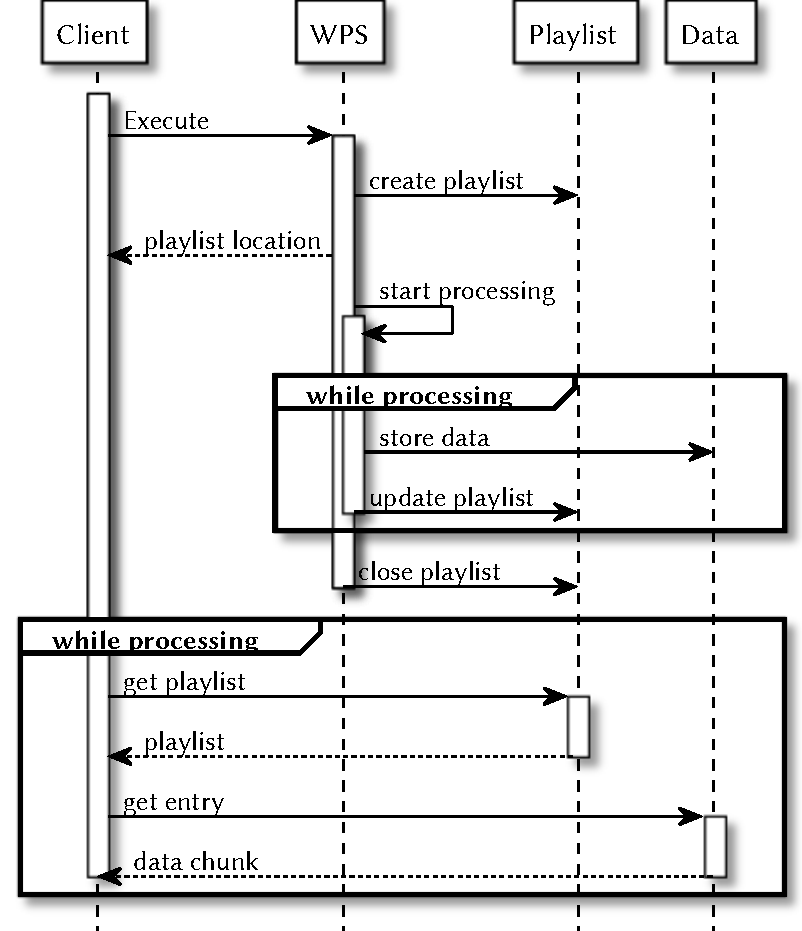
\includegraphics[width=0.54225352112676062\linewidth]{figures/sequence-diagramm-previous.pdf}
		\caption{\label{fig:sd:previous}Sequence diagram of the playlist-based streaming enabled WPS \citep{foerster2012live}.}
	\end{figure}

	Input parameters may also be supplied using a playlist file. The coordination of several streaming inputs is either not possible or heavily depending on the streaming enabled process. A process accepting two ore more streamed data sets has to decide which data chunks it has to combine. Even the simplest case of combining chunks with the same index of both streams can have serious implications in the use case of live analysis. If a data chunk gets lost, either due to hardware or network failure, the process will combine chunks that are not related. In continuous processes this error can not be detected because two indefinite streams of data will always have matching indices. Use cases, in which the rate of incoming data differs between streams or in which data chunks depend on other chunks, are very hard to model and will result in highly specialized processes. These models depend not only on the structure and format of input data, but also on the data source, and thus the incoming rate of the data. By this, generic solutions, that convert existing \ac{WPS} processes into streaming enabled processes, are hard to develop, and most streaming enabled processes may not be used in contexts apart from the one that it was developed for.

	Moreover, realizing streaming by continuous polling of playlists is highly inefficient. Neither can the client know the rate output data is produced nor can the \ac{WPS} process know at which rate input data becomes available. By polling at a too slow rate the arrival of data chunks may be missed, which results in a slower process execution, and by polling at a too high rate, network and computation resources are wasted. Adaptive polling rates may be a solution for this problem, but are useless in cases, where the rate of incoming data changes across the process execution. In contrast to transporting data from the server to the client, for which the playlist concept was originally developed in the context of media streaming, the usage of playlists to transport data from the client to the server is additionally questionable. Clients need the capability to publish files as resources, which are accessible using an URL (e.g. on a FTP or HTTP server). In a web browser environment, a JavaScript client is only able to do this using an external service that stores the data and maintains the playlist. A pure JavaScript browser client is not able to use streaming inputs in this playlist-based streaming \ac{WPS} approach. The implementation of this approach is additionally limited. Input parameter data streams are not implemented and process implementations have to split inputs to create output streams (see \cref{fig:streaming}c). Splitting spatiotemporal data into smaller chunks is not as trivial as e.g. splitting an audio or video stream into single frames. By this, the process implementations become heavily format dependent and dependencies between data chunks can only be expressed as part of the data, and in a format, that the process is able to understand and to handle. Also this approach requires a reimplementation of already existing processes to achieve streaming outputs.

	% TODO: daten hängen von ihrer umgebung ab: quelle?
	A streaming enabled \ac{WPS} should extend the traditional processing paradigm (see \cref{fig:streaming}a) to enable input only streaming (\cref{fig:streaming}b), output only streaming (\cref{fig:streaming}c), and full input/output streaming (\cref{fig:streaming}d). For this, it should be possible to supply input parameters subsequently and to publish output data chunks as they become available. To accomplish this, a streaming enabled \ac{WPS} should not rely on inefficient polling techniques, in which the server or client is requesting a resource continuously over time, but should rely on true streaming technologies that offer a full-duplex communication channel between client and server. Streaming enabled processes should be accessible from the same environments as conventional \ac{WPS} processes. This especially includes web browser environments that are particularly restricted in their possibilities. A streaming enabled \ac{WPS} process should rely on existing, widely known and standardized technologies, it should be especially as interoperable as possible to the \ac{WPS} specification, but should not compromise streaming functionality by enforcing incompatible standards. As spatiotemporal data and its processing and analysis often can not be treated independently from surrounding data, dependencies between streamed data chunks have to be considered. This will require the streaming enabled process to be able not only to operate on sequential data but also be able to allow, to some degree, random access to the data. Despite handling of dependencies between spatiotemporal features should be considered, processes and algorithms that require global knowledge of the data set, may not profit from streaming and should not be considered relevant for a streaming enabled \ac{WPS}. The system should be as generic as the existing \ac{WPS} specification, so it should not rely on specific data formats and allow easy chaining of streaming processes. As possible use cases include not only live analysis of data, but also the processing of large data set, data chunks should be processed in parallel if possible. As this may result in an undefined order of outputted data chunks, clients need to be able to correlate output data chunks with the input parameter chunks. Existing \ac{WPS} processes should be easily converted to streaming enabled processes, without the need to develop them from scratch.

	The following sections should introduce a approach for a Streaming \ac{WPS}, that will fulfill the above requirements. As seen in previous approaches, the constraints imposed by the \ac{WPS} specification are too strict to implement a standard compatible streaming enabled WPS fulfilling the requirements. Previous solutions compromised functionality for the sake of (incomplete) compatibility with the inflexible standard. In order to enable true, browser compatible streaming, the approach presented in thesis will break out of the constraining \ac{WPS} standard and develop a message based architecture using WebSockets to accomplish true full-duplex streaming of data while reusing terminology and technology specified by the \ac{WPS} standard.

	\section{Protocol}
		As the \ac{WPS} specification is not flexible enough to model a full streaming scenario, the \ac{WPS} needs to be bypassed. In order to accomplish this, a more flexible interaction model was developed, which extends the conventional processing approach. This protocol is message based and enables full-duplex stream processing of spatiotemporal data. A \emph{streaming enabled algorithm} is a \ac{WPS} algorithm that supports the here defined protocol while a \emph{streaming process} is the identifiable instance of an algorithm, created by executing the streaming enabled algorithm using the \ac{WPS} \emph{Execute} operation. The streaming process is the core of the Streaming \ac{WPS} and receives subsequent inputs and will emit intermediate results. The execution of the streaming enabled algorithm is fully supported by the \ac{WPS} specification, whereas all interaction with the streaming process is not part of the standard. To communicate with the streaming process, the client needs information on how to connect to the process. As the \ac{WPS} specification does not allow subsequent outputs, the call of the \emph{Execute} operation will return immediately to transport this information to the client, and can not persist over the lifetime of the streaming process.

		To enable a full duplex communication with the streaming process, WebSockets will be used to transport messages. They are needed to \emph{push} messages to clients instead of letting the clients constantly request updates.

		\begin{figure}[!htb]
			\centering
			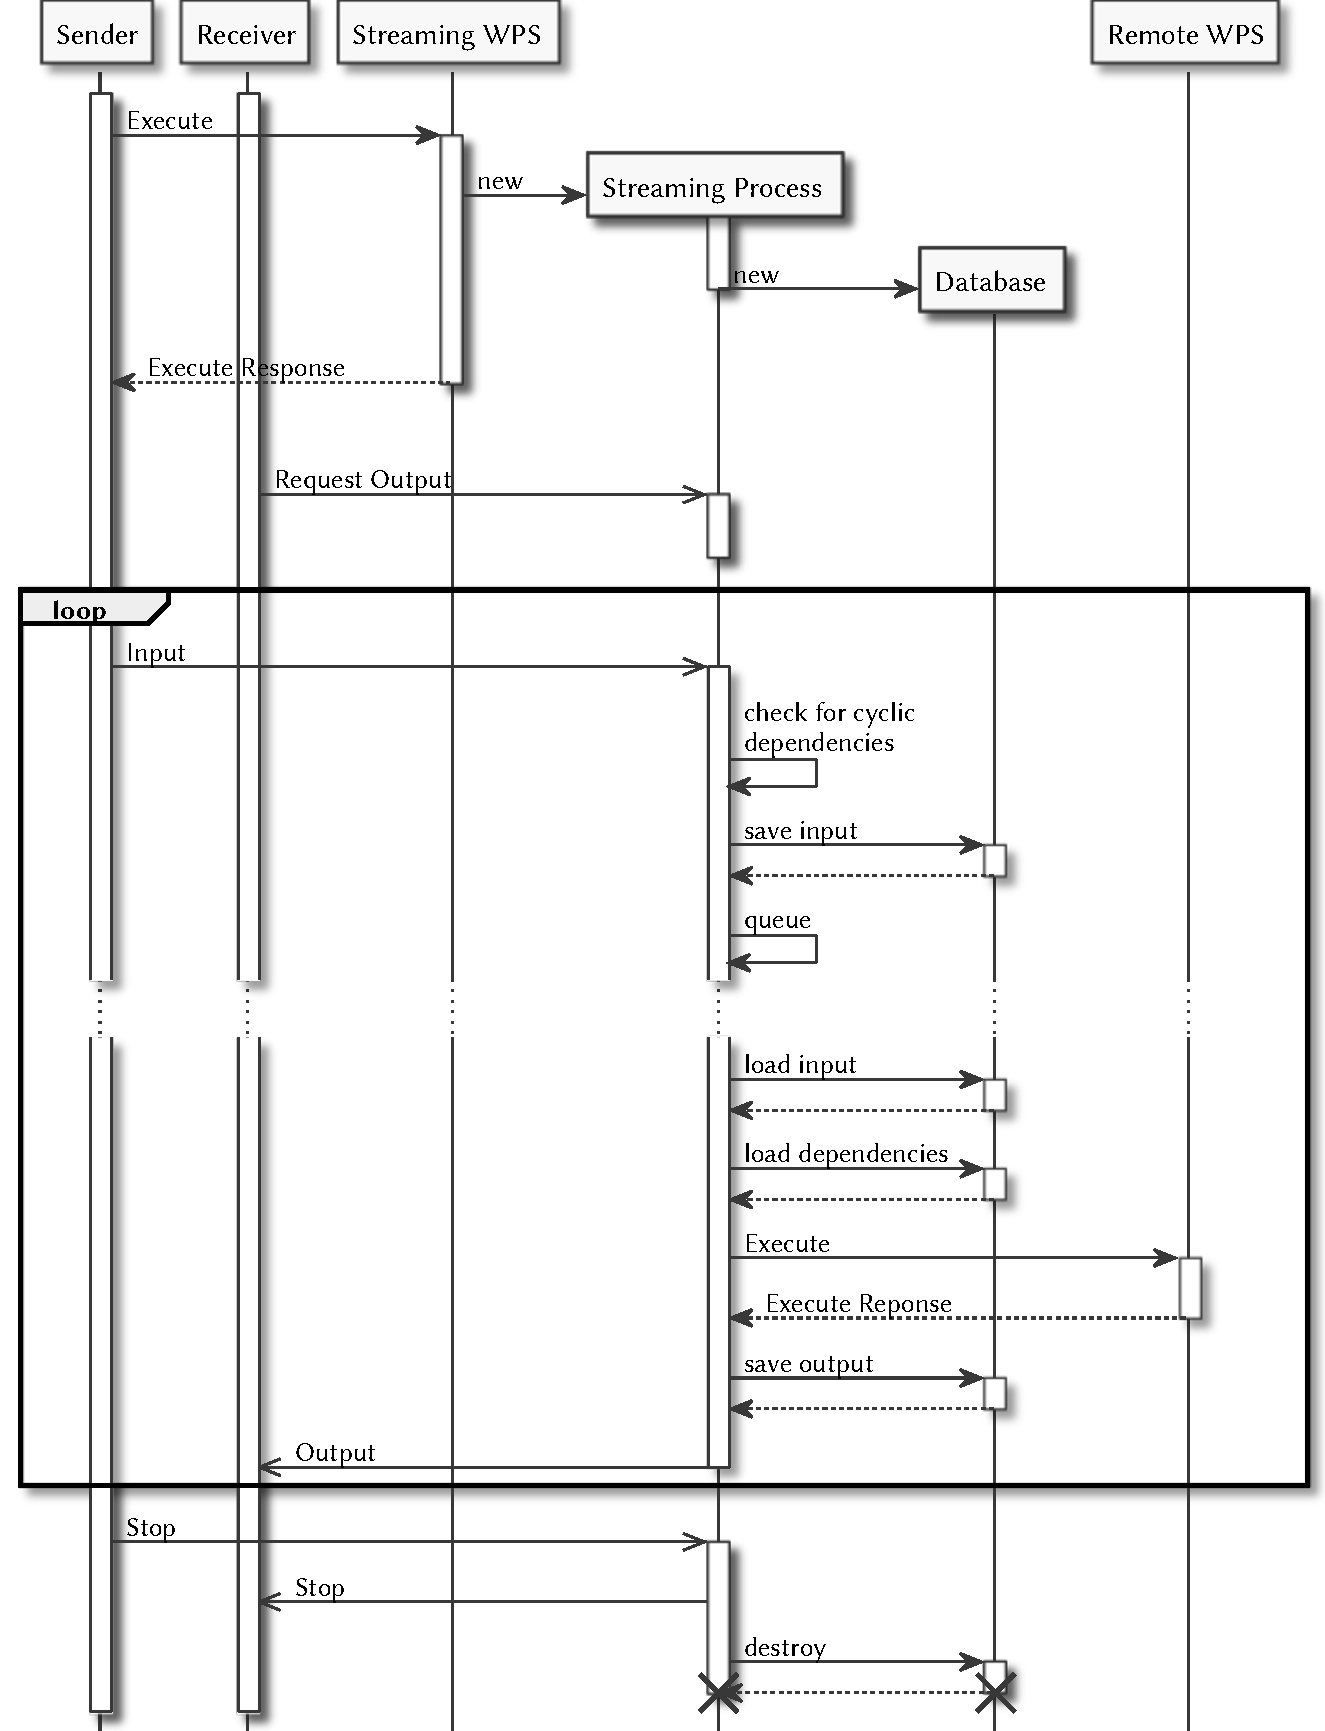
\includegraphics[width=0.82253521126760565\linewidth]{figures/sequence-diagramm-swps.pdf}
			\caption{\label{fig:sd:swps}Sequence diagram of typical interaction pattern with a streaming enabled WPS algorithm using two distinct clients for sending and receiving data.}
		\end{figure}

		The detailed interaction protocol is depicted in \cref{fig:sd:swps}. A client (\emph{Sender}) issues an \emph{Execute} to a streaming enabled WPS algorithm (\hyperref[fig:sd:swps]{step~1}). The algorithm instantiates a delegate (\hyperref[fig:sd:swps]{step~2}) that is responsible for processing data chunks, and a streaming process (\hyperref[fig:sd:swps]{step~3}) that is responsible for client interactions and task scheduling. The Execute response will contain the necessary details to connect to the streaming processes, such as the the identifier of the streaming process and the WebSocket endpoint URL (\hyperref[fig:sd:swps]{step~4}).

		With these details a client can connect directly to the streaming process bypassing the \ac{WPS} interface. In \hyperref[fig:sd:swps]{step~5} another client\footnote{Even though sender and receiver are two different entities in this diagram, there are no restrictions imposed to the amount of clients, either senders or receivers, or their nature (senders may also be receivers).} (\emph{Receiver}) connects to the streaming process and subscribes to the future outputs of the process. By this, the client does not need to constantly issue requests to the streaming process to check for new outputs, but receives outputs automatically as long as the receiving client stays connected using the WebSocket.
		After this, one or multiple clients start sending chunks of data as input parameters to the streaming process (\hyperref[fig:sd:swps]{step~6}). The clients may open a new connection for every input or use the same connection over the lifetime of the streaming process. The streaming process checks the inputs for validity (\hyperref[fig:sd:swps]{step~7}) and queues them for processing (\hyperref[fig:sd:swps]{step~8}).
		Processing takes places asynchronously in parallel manner and there is no guarantee of order (besides restrictions imposed by dependencies, see \cref{sec:stream:input:reference,sec:stream:dependencies}). When there are free capacities to process the data and all other requirements are met, the delegate is tasked to process the data (\hyperref[fig:sd:swps]{step~9}). The delegate implementation can return an intermediate result in \hyperref[fig:sd:swps]{step~10}, which is forwarded to all registered receivers in \hyperref[fig:sd:swps]{step~11}.
		\hyperref[fig:sd:swps]{Steps~6~to~11} may be repeated indefinitely (e.g. live analysis of data) or until the sending client has no more inputs to feed. As the streaming process would wait in this case forever (or at least until some timeout interferes), the client has to stop the streaming process explicitly (\hyperref[fig:sd:swps]{step~12}).
		This causes the streaming process to stop accepting inputs, to process all not yet processed inputs, and to request a last potential output from the delegate (\hyperref[fig:sd:swps]{step~13~and~14}), which is forwarded to all listening clients (\hyperref[fig:sd:swps]{step~15}). After this, it destructs the delegate (\hyperref[fig:sd:swps]{steps~16~and~17}) and notifies all registered listeners, that no further outputs will become available by forwarding the stop message (\hyperref[fig:sd:swps]{step~18}) to the clients. The streaming process will destroy itself after this. A detailed description of the various messages of this protocol can be found in \cref{sec:streaming:messages}.

		The protocol permits various streaming usage scenarios. A delegate that produces an output for every input message creates a full input/output streaming process (see \cref{fig:streaming}d). A delegate that produces only a final output results in an input only streaming process (see \cref{fig:streaming}b). By suppling a single input message and repeating step 11, a suitable delegate may create an output streaming process (see \cref{fig:streaming}c) and, although not reasonable, even the traditional processing approach depicted in \cref{fig:streaming}a can be simulated by passing all inputs in a single input message and producing a single output message.

		Using message provoked streaming iterations (the combination of an input message, its processing and (optional) output message) allows the use of multiple streaming inputs and outputs. In contrast to previous approaches it is possible for the streaming process to relate these to a single processing iteration without any knowledge of their semantics because the client encapsulates them in a single message.

		\begin{figure}[!htb]
			\centering
			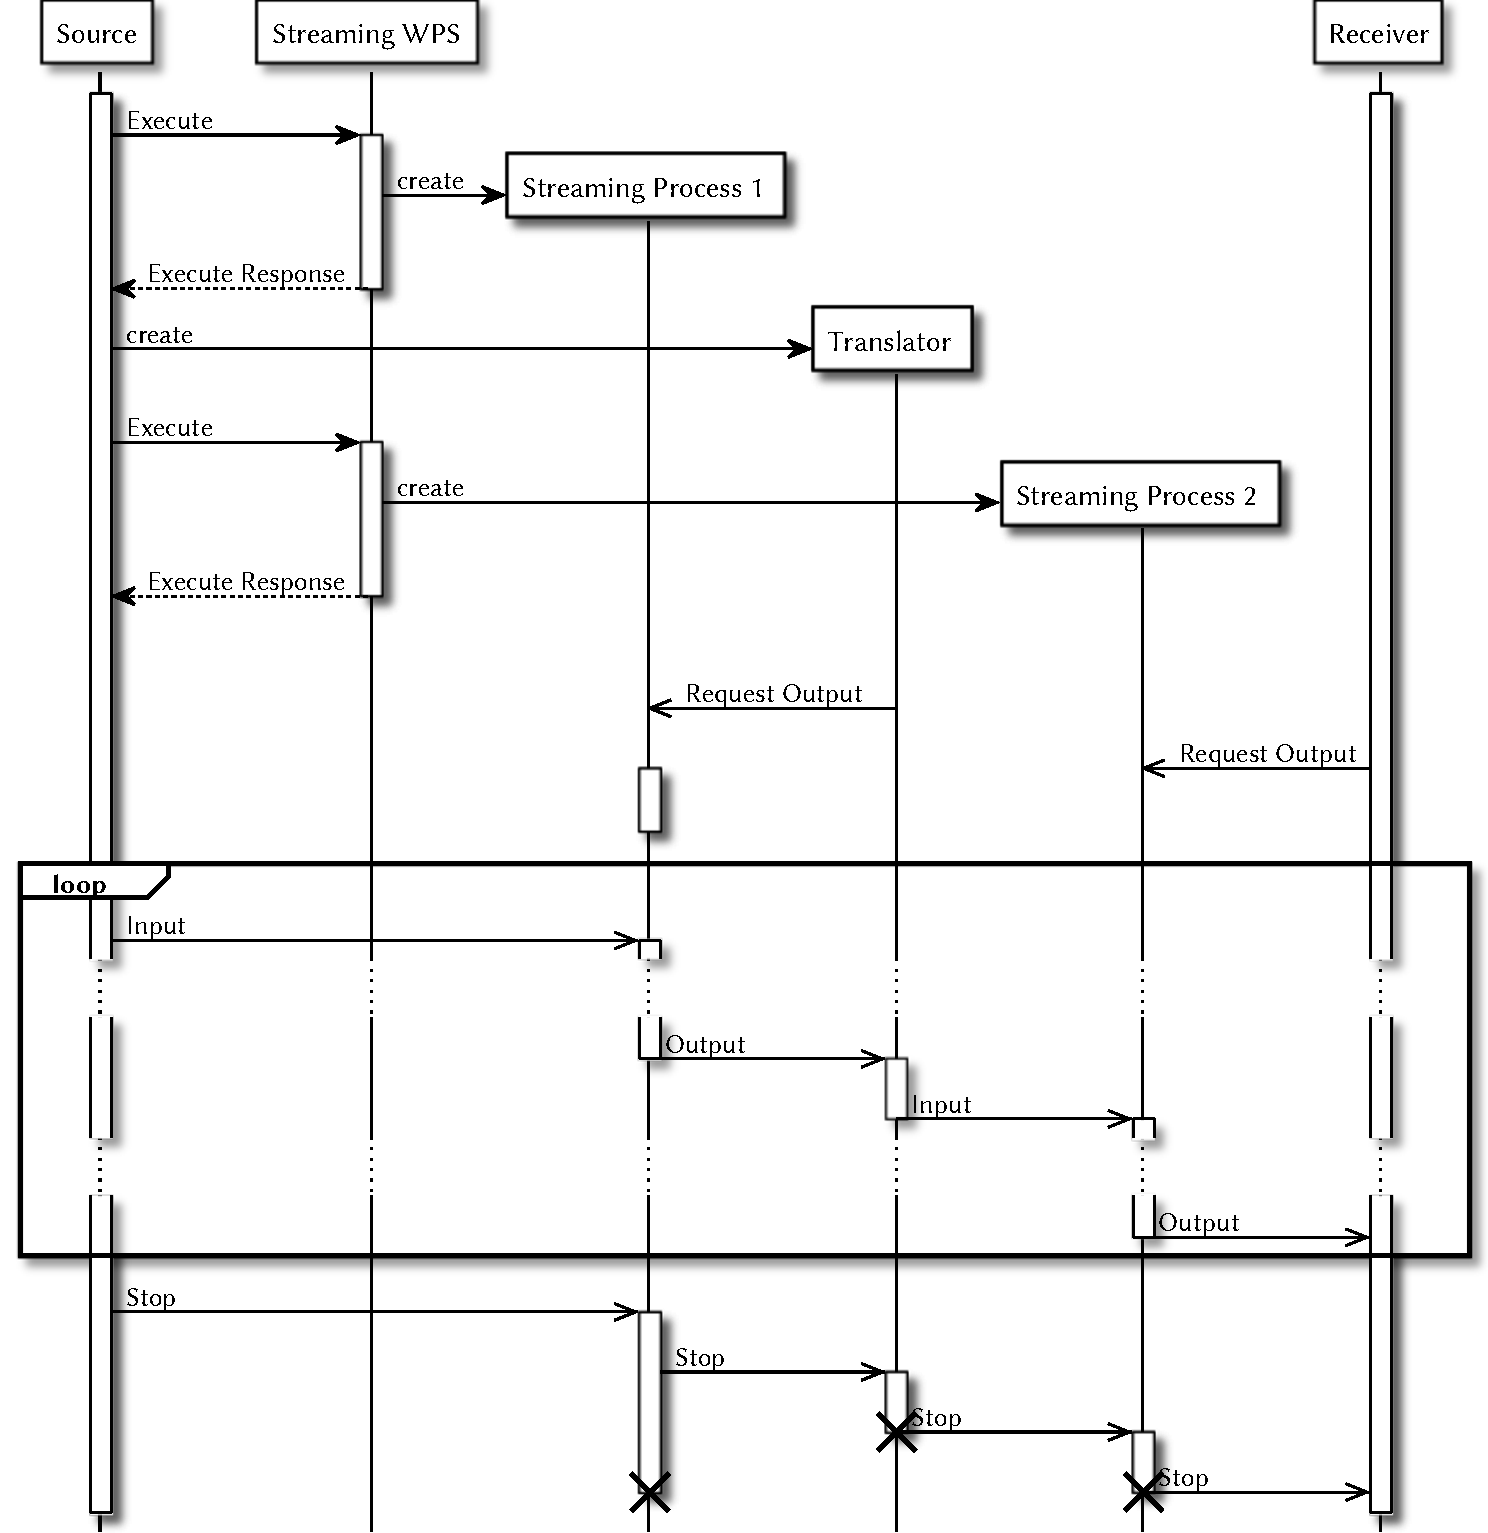
\includegraphics[width=1\linewidth]{figures/sequence-diagramm-chain.pdf}
			\caption{\label{fig:sd:chain}Sequence diagram of chaining two streaming processes using a generic mediator between the processes to translate output to input messages.}
		\end{figure}

		The protocol also enables the chaining of processing steps. This can be realized in two ways: on the one hand, a delegate itself may represent a \ac{WPS} process chain and thus chain every processing step, or, on the other hand, several streaming processes are chained. A simple mediator is translating input messages to output messages (see \cref{fig:sd:chain}). This mediator can be realized using a dedicated streaming enabled algorithm accepting an input/output mapping and the connection parameters of the streaming processes to connect. After requesting the outputs of the source streaming process, it can translate every output message to an input message and forward the stop message. A receiving client will connect to the second streaming process and receives the data process by the chain. By requesting the outputs of the first streaming process, even intermediate results of the chain are accessible.

	\section{Messages}
		\label{sec:streaming:messages}
		To fulfill the above defined protocol several messages have to be exchanged between sender, streaming process and receiver. In order to correlate input and outputs or to show the source of an error, the message format has to have a concept of message references. WebSockets do not have such a concept as it is only a thin layer on top of TCP, that introduces handshake and addressing mechanism to be compatible with HTTP and a minimal framing of messages. This framing is merely needed to establish a message-based instead of a stream-based protocol, as the latter would make it hard to differentiate between individual messages \citep{ietf:rfc6455}. To enable referencing of messages, and by this a asynchronous reply mechanism, another layer is needed. As the \ac{WPS} is mostly based on \ac{XML}, the message format should also be \ac{XML} based. This enables the usage of large parts of the \ac{WPS} schema and allows the reuse of many components written to interact with the \ac{WPS}.

		The widely known SOAP protocol \citep{w3c:soap1}, which may also be used as an optional binding of the \ac{WPS} \citep{ogc:wps} and thus can be easily adopted, is an ideal candidate for this. In combination with \ac{WSA} \citep{w3c:wsa} it creates an \ac{XML} based message framework, that allows asynchronous requests and responses over an arbitrary protocol. Besides introducing a concept of addressing and routing of messages (that will not be used in the Streaming \ac{WPS}), one can assign a globally unique identifier to any message using \ac{WSA}, that can be referenced with arbitrary semantics (e.g. reply).

		The Streaming \ac{WPS} defines seven SOAP messages:

		\subsection{Input Message}
			Input messages are used by clients to supply subsequent inputs to a streaming iteration of a streaming process. They loosely resemble a \ac{WPS} Execute request by consisting of any number of inputs and a identifier, which references the streaming process to which the inputs should be supplied. An example can be seen in \cref{lst:streaming:message:input}, possible inputs can be seen in \cref{sec:streaming:input}.
			\lstinputlisting[label={lst:streaming:message:input},
							 caption={[Example for a Streaming WPS input message.]Example for a Streaming WPS input message (see \cref{sec:xmlnamespaces} for omitted XML namespaces).},
							 language=XML]{listings/streaming-message-input.xml}
		\subsection{Output Messages}
			Output messages are used by the streaming process to transport intermediate results at the end of a streaming iteration or a final result at the end of the streaming process to listening clients. They loosely resemble a \ac{WPS} Execute response by containing a arbitrary number of outputs and the identifier of the process, that produced the outputs. Output messages containing intermediate result are replies to their corresponding input message and reference them using \ac{WSA}. If the processing used the output of any other streaming iteration (see \cref{sec:stream:input:reference,sec:stream:dependencies}) the corresponding output messages are also referenced. An example can be seen in \cref{lst:streaming:message:output}.
			\lstinputlisting[label={lst:streaming:message:output},
							 caption={[Example for a Streaming WPS output message.]Example for a Streaming WPS output message (see \cref{sec:xmlnamespaces} for omitted XML namespaces).},
							 language=XML]{listings/streaming-message-output.xml}
		\subsection{Output Request Message}
			A output request message is used by a client to let a streaming process know, that it would like to receive outputs from the process. There is no direct counter part in the \ac{WPS} specification but the concept is similar to the continuous request of the \ac{WPS} response during a asynchronous process execution. As WebSockets offer a full-duplex messaging channel a continuous polling of outputs is not needed, but the streaming process can push outputs directly to listening clients. To initialize this listening, the client registers to one or more streaming processes using their corresponding identifiers. An example can be seen in \cref{lst:streaming:message:output-request}.
			\lstinputlisting[label={lst:streaming:message:output-request},
							 caption={[Example for a Streaming WPS output request message.]Example for a Streaming WPS output request message (see \cref{sec:xmlnamespaces} for omitted XML namespaces).},
							 language=XML]{listings/streaming-message-output-request.xml}
		\subsection{Stop Message}
			As streaming process can run indefinitely long, input supplying clients need to be able to let the streaming process know, that there will be no further inputs that become available. To achieve this a stop message (see \cref{lst:streaming:message:stop}) is send to the streaming process. The process will propagate the stop message to all listening clients to let them know there will be no further outputs. Before the stop message is propagated all streaming iterations, that are not yet processed will be finished but the process will not accept any further inputs. If there are still unresolved dependencies (see \cref{sec:stream:input:reference,sec:stream:dependencies}) the streaming process will fail with an error message.
			\lstinputlisting[label={lst:streaming:message:stop},
							 caption={[Example for a Streaming WPS stop message]Example for a Streaming WPS stop message (see \cref{sec:xmlnamespaces} for omitted XML namespaces).},
							 language=XML]{listings/streaming-message-stop.xml}
		\subsection{Error Message}
			Errors are transported, as in the \ac{WPS} specification, using \ac{OWS} exception reports \citep{ogc:wps}. If the delegate of a process fails or a supplied input message can not be processed due to whatever conditions, the error is propagated to listening clients. The error is always send to the client that send the message causing the error (if the client is still connected) and in case the error is caused during the execution of a streaming iteration, also to all listening clients, that registered through a output request message. In contrast to failures during input validation, due to constraints imposed by dependencies (see \cref{sec:stream:input:reference,sec:stream:dependencies}), errors raised during the execution of a streaming iteration can not be compensated, but will stop the streaming process. The causing message of a failure may be obtained from the reply relation encoded using \ac{WSA}. An example of an error message can be found in \cref{lst:streaming:message:error}.
			\lstinputlisting[label={lst:streaming:message:error},
							 caption={[Example for a Streaming WPS error message.]Example for a Streaming WPS error message (see \cref{sec:xmlnamespaces} for omitted XML namespaces).},
							 language=XML]{listings/streaming-message-error.xml}
		\subsection{Describe \& Description Message}
			Describe messages are directly adopted from the \ac{WPS} Describe Process operation. Due to conditions described in \cref{sec:stream:processdescription} a client needs to be able to retrieve a description from a running streaming process. The message simply contains the identifier of the process the clients wants to have the description from. An example for this process can be seen in \cref{lst:streaming:message:describe}.
			\lstinputlisting[label={lst:streaming:message:describe},
							 caption={[Example for a Streaming WPS describe message.]Example for a Streaming WPS describe message (see \cref{sec:xmlnamespaces} for omitted XML namespaces).},
							 language=XML]{listings/streaming-message-describe.xml}
			The reply resembles a \emph{DescribeProcess} response and is encoded in a description message referencing the describe message and containing the streaming process description and (see \cref{lst:streaming:message:description}).
			\lstinputlisting[label={lst:streaming:message:description},
							 caption={[Example for a Streaming WPS description message.]Example for a Streaming WPS description message (see \cref{sec:xmlnamespaces} for omitted XML namespaces).},
							 language=XML]{listings/streaming-message-description.xml}

	\section{Input Types}
		\label{sec:streaming:input}
		The aforementioned requirements imply three different types of input for a Streaming Process. They differ in the aspect of time (\emph{When are they supplied?}) and scope (\emph{Where are they used?}). Besides that all of them are based on the very same input types the \ac{WPS} standard defines (see \cref{sec:wps}).
		\subsection{Streaming Inputs}
			\label{sec:streaming:input:streaming}
			The first and most obvious type of input are streaming inputs. They are provided for a single streaming iteration and will only be used in that iteration representing the core of streaming enabled processing (see \cref{lst:streaming:input:streaming}).

			\lstinputlisting[label={lst:streaming:input:streaming},
							 caption={[Example for a Streaming WPS streaming inputs.]Example for a Streaming WPS streaming inputs (see \cref{sec:xmlnamespaces} for omitted XML namespaces).},
							 language=XML]{listings/streaming-input-streaming.xml}


			A conventional algorithm to compute the histogram of a raster (e.g. a satellite image) needs the complete raster as a single complex input for processing. A streaming enabled variant would split the raster in several smaller tiles and supply each of them in a single input message to the streaming process. The algorithm can process each tile on it's own and update the global histogram. Besides that the process does not have to store the complete raster, it is also able to output intermediate histograms to the client.

		\subsection{Static Inputs}
			\label{sec:stream:input:static}
			Algorithms that operate on a streaming input often need inputs that are common to every iteration. It would be redundant and inefficient to transfer inputs like configuration parameters in every input message for every streaming iteration. For this, the concept of static inputs needs to be introduced. Static inputs are parameters that are supplied when a streaming process is created and apply to every streaming iteration (see \cref{lst:streaming:input:static}). While the streaming process handles a streaming iteration, the static inputs are merged with the inputs of the causing input message and transparently supplied to the process's delegate. This way a conventional process can be easily converted into a streaming enabled process. Additionally static inputs can be handled separately to configure a streaming process' delegate when it is created.

			\lstinputlisting[label={lst:streaming:input:static},
							 caption={[Example for a Streaming WPS static inputs.]Example for a Streaming WPS static inputs (see \cref{sec:xmlnamespaces} for omitted XML namespaces).},
							 language=XML]{listings/streaming-input-static.xml}

			For example, a traditional process implementation of the Douglas-Peucker algorithm \citep{douglas1973algorithms} would require a feature collection and a $\epsilon$ value as inputs. In a streaming environment, one would model the $\epsilon$ input as a static input supplied at process creation and stream the feature collection as single features in streaming inputs. Other examples are a coordinate transformation process, that accepts a feature collection and a target \ac{CRS} or a buffer algorithm that accepts a feature collection and a buffer size. Buffer size and \ac{CRS} would be supplied as static inputs and the feature collection would be split into several streaming inputs and supplied in independent streaming iterations.

		\subsection{Reference Inputs}
			\label{sec:stream:input:reference}
			While streaming offers no real benefit to algorithms that require global knowledge of the data set, there are often cases where algorithms only require knowledge about few other chunks of the data set or even only about the result of their processing. To model these dependencies between streaming iterations, reference inputs can be used (see \cref{lst:streaming:input:reference}). These reference the output of another, previous or upcoming, iteration as an input parameter. Reference inputs break out of the conventional non-random access paradigm of streaming and allow a semi-random access processing of a data set. Inputs are described by referencing the corresponding output identifier and the input message that has or will produce the output data. The order of incoming input messages is irrelevant to the use of reference inputs, as input messages referencing not yet available outputs will be delayed until they can processed (see \cref{sec:stream:dependencies}).

			\lstinputlisting[label={lst:streaming:input:reference},
							 caption={[Example for a Streaming WPS reference input.]Example for a Streaming WPS reference input (see \cref{sec:xmlnamespaces} for omitted XML namespaces).},
							 language=XML]{listings/streaming-input-reference.xml}

			A conventional algorithm to analyze a river system, in which each processing of a river depends on the processing results of the rivers flowing into it, the complete river system data set would be supplied as a single input parameter. In a streaming enabled process, each river would be supplied as a streaming input. The output of the rivers which a river depends on would be supplied as additional reference inputs.
		\subsection{Polling inputs}
			\label{sec:stream:input:polling}
			The last category of possible input types for a streaming \ac{WPS} are polling inputs. These inputs are continuously polled from an external resource and a new streaming iteration would be started, when new inputs become available. Polling inputs would be supplied at process creation time and would contain a reference to an external resource, that is requested continuously. To not miss inputs, when they become available, a playlist file, as described in previous approaches \citep{foerster2012live} would be need. The implementation of polling inputs as part of this streaming \ac{WPS} specification would present the very same issues, that were criticized in previous approaches: how one can define the polling frequency used to retrieve the playlist? How can multiple polling inputs be declared, and how would they be combined by the streaming \ac{WPS}? For this reason the Streaming \ac{WPS} will not implement polling inputs. These input types are by far better handled on client side, as the client typically knows of the rate data becomes available and so can choose an appropriate polling frequency and also is able to coordinate multiple polling inputs by having a deeper understanding of their affiliation. Polling inputs could be implemented as shown in \cref{fig:sd:polling}: the client polls a data provider (e.g. a \ac{SOS}) to check if new data is available and convert this data into a streaming input for the Streaming \ac{WPS}.
			% TODO SES/SAS/etc?
			\begin{figure}[!htb]
				\centering
				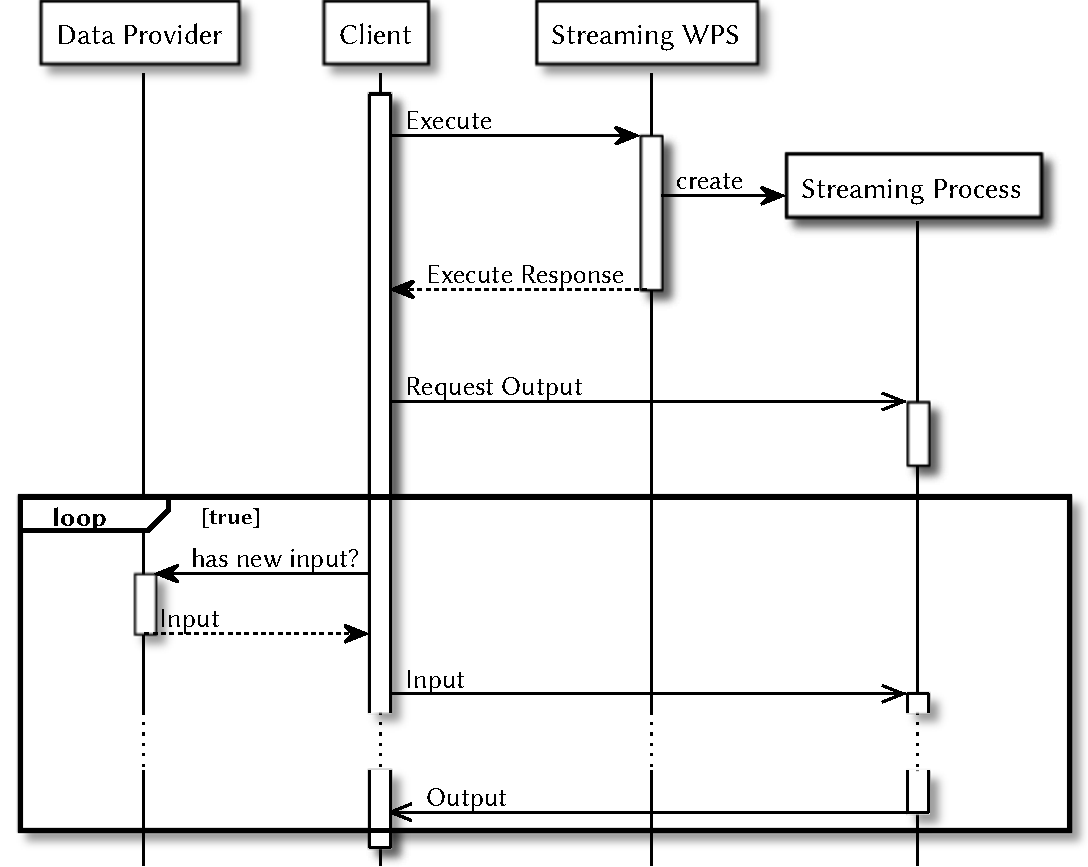
\includegraphics[width=0.73521126760563382\linewidth]{figures/sequence-diagramm-polling.pdf}
				\caption{\label{fig:sd:polling}Sequence diagram of how to implement polling inputs for a streaming enabled WPS algorithm.}
			\end{figure}

	\section{Dependencies}
		\label{sec:stream:dependencies}
		The definition of Reference Inputs in \cref{sec:stream:input:reference} implies a mechanism to resolve dependencies and to order the execution of streaming iterations. These are considered as tasks and can declare dependencies to other streaming iterations either by mapping an input to the output of another streaming iteration or by declaring a explicit dependency on another streaming iteration.

		Dependencies can be best modeled using a \ac{DAG}. A \ac{DAG} is a structure $D=(V, E)$ consisting of a set of vertices (or nodes) $V$ and edges (or arcs) $E$ where every edge $e\in E$ is a ordered pair $v_1 \rightarrow v_2$ with $v_1, v_2 \in V$. The distinct vertices $v_1,\dots,v_n\in V$ are called a path if for all successive vertices $v_i, v_{i+1}$ exists a edge $v_i \rightarrow v_{i+1} \in E$. A directed graph is called acyclic if there exists no path in $G$ with $v_1 = v_n$ \citep{jungnickel2012graphs}. A subgraph of a graph is the graph $G' = (V', E')$ with $V'\subseteq V$ and $E' = \{v_1 \rightarrow v_2 \in E | v_1, v_2\in V'\}$. Two subgraphs $G_1 = (V_1, E_1), G_2 = (V_2, E_2)$ are independent if $V_1 \cap V_2 = \emptyset$ and there exists no edge $v_1\rightarrow v_2\in E$ with $v_1\in V_1 \wedge v_2\in V_2$ or $v_2\in V_1 \wedge v_1\in V_2$.

		In a dependency graph, vertices represent a task, package or other entity that has dependencies and edges represent these dependencies ($v_1$ depends on $v_2$). Dependency graphs have to be acyclic as a cycle would introduce a cyclic dependency, that can not be resolved.

		\begin{figure}[!htb]
			\centering
			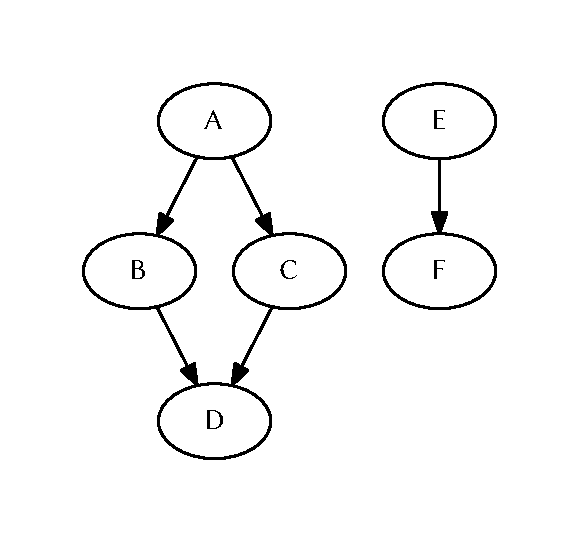
\includegraphics[width=0.44694533762057875\linewidth]{figures/unordered-graph.pdf} % 98x92
			\caption{\label{fig:graph:unordered}Example for a dependency graph consisting of two independent subgraphs. Arrows denoting a dependency between the nodes.}
		\end{figure}

		A system containing the tasks $A, B, C, D, E, F$ and the dependencies $A\rightarrow B, A\rightarrow C, B\rightarrow D, C\rightarrow D$ and $E\rightarrow F$ will result in a \ac{DAG} consisting of two independent subgraphs (see \cref{fig:graph:unordered}).

		The execution order of a dependency graph can be derived from the topological ordering of the graph: a ``topological ordering, $ord_D$, of a directed acyclic graph $D = (V, E)$ maps each vertex to a priority value such that $ord_{D}(x) < ord_{D}(y)$ holds for all edges $x \rightarrow y \in E$'' \citep{pearce2007dynamic}, a possible execution order is the list of all vertices sorted by descending $ord_D$. The topological order of a \ac{DAG} can be computed using e.g. \ac{BFS} in linear time \citep{cormen2001introduction}. In most cases the topological ordering is not unique, \cref{fig:graph:ordered} shows one possible execution order for the before mentioned graph.

		\begin{figure}[!htb]
			\centering
			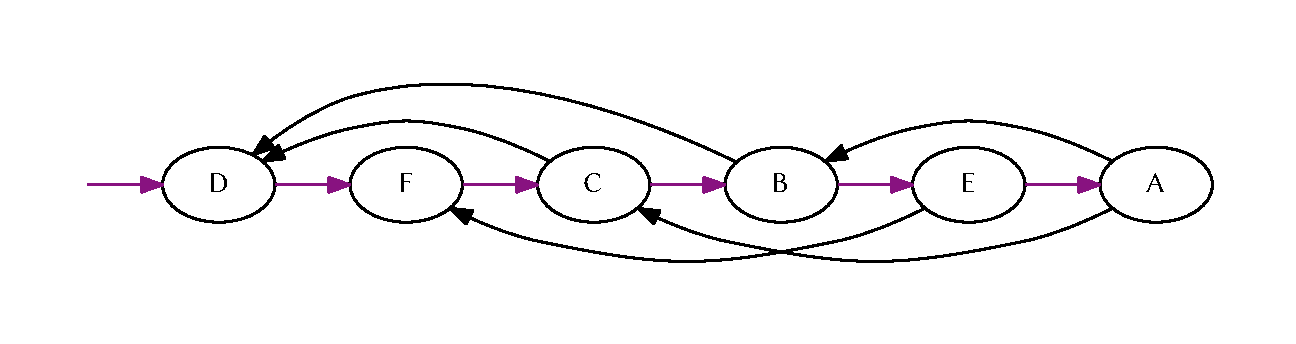
\includegraphics[width=1\linewidth]{figures/ordered-graph.pdf} % 219x58
			\caption{\label{fig:graph:ordered}Possible execution/topological order of the dependency graph in \cref{fig:graph:unordered}. Black arrows represent dependence to another vertex, colored arrows the execution order.}
		\end{figure}

		In contrast to conventional dependency systems like package managers the Streaming \ac{WPS} can not operate on a static graph of dependencies but on a graph to which vertices and edges are added constantly. Conventional topological sorting algorithms have to recompute the ordering for every insertion from scratch which will have a big performance impact for the scenario of a great number of small streaming iterations. There exist few dynamic topological sort algorithms that will maintain the topological order across edge and node insertions and will only recompute the ordering if necessary.

		Most dependency graphs generated using the Streaming \ac{WPS} will probably consist of multiple independent subgraphs, no dependencies at all would be the most extreme example, or quite sparse graphs. For this the algorithm described by \citet{pearce2007dynamic} seems to be appropriate. Even it is theoretically it is inferior to other algorithms for dynamic topological sorting \citep[e.g. ][]{alpern1990incremental,marchetti1996maintaining}, in practice it especially performs better on sparse graphs and on dense graphs only a constant factor slower than other algorithms \citep{pearce2007dynamic}. %wörtliches zitat?

		Dependencies are of particular importance in case of execution failures. If the computation of a streaming iteration fails for whatever reason, all iterations, that directly or indirectly depend on this iteration can not complete. As this also holds true for iterations, that are supplied at a later time in the streaming process, the process can not proceed ignoring the error. Due to this every error that occurs during the execution of a streaming iteration result in the termination of the streaming process.
		Dependencies also have a special meaning at the end of a streaming process, when a stop message is sent to notify the streaming process to accept no further inputs and finish pending streaming iterations. At this point all dependencies need to be able to be satisfied, which implies that all referenced input messages have been sent to the streaming process. In case a referenced input message the service is not able to complete gracefully and fail. As references to future streaming iterations are allowed, prior to this point, it is not possible for the Streaming \ac{WPS} to determine if reference may not be fulfilled. As the service is not able to fail fast for incorrect references, clients using dependencies between streaming iterations have to pay careful attention to references.

		It should also be noted, that for a streaming process the smallest unit, that can be referenced, is the output of a streaming iteration. Format specific references, e.g. to a particular feature inside a feature collection, are not possible using this protocol and streaming process implementations need to be designed to not need smaller components or have to deploy a own referencing strategy (e.g. by additionally supplying an additional input to identify the feature of the referenced collection). But, as this results in superfluous transfer of data, such solutions should be avoided. One may point out, that there is no way to reference input parameters of other streaming iterations, but this use case should be already covered by the \ac{WPS}' own input reference parameters (see \cref{sec:streaming:input}).

	\section{Process Description}
		\label{sec:stream:processdescription}
		The conventional process description mechanism of the \ac{WPS} is not sufficient to describe streaming processes.

		It consists of a \emph{DescribeProcess} request issued to the \ac{WPS} and the retrieval of one or more process descriptions of the specified process. These descriptions contain detailed descriptions of input and output parameters of the process and information about the supported formats, units of measurement or coordinate reference systems of each parameter. They also include details about allowed values, default value and multiplicity of input parameters \citep{ogc:wps}.

		Because the Streaming \ac{WPS} uses the \ac{WPS} interface only to start a Streaming Process and the \ac{WPS} interface does not provide any extension points for process descriptions, the \emph{DescribeProcess} operation can only be used to describe the starting process, but not the input or output parameters of a streaming process.

		In case of generic processes, e.g. processes that delegate to other \ac{WPS} processes, information about input and output parameters is not even available prior to the execution of the streaming process. Furthermore input parameter cardinalities may change due to the use of static inputs. By this a valid input parameter for a delegate process may not be used in subsequent inputs because the maximal occurrence of the parameter is already exhausted using static input parameters. By this a process description for a streaming process will always be instance specific and can not be generated by the associated \ac{WPS} process.

		With knowledge of the delegate process a client may have enough information to facilitate the streaming process but for other streaming process there is no way for a generic client to know the input parameters of the process.

		To compensate this shortcoming a method is needed to describe a Streaming Process instance at runtime.

	\section{Implementation}
		The Streaming WPS was prototypically, but feature complete implemented as a module for the \ftn WPS implementation. Besides offering a framework to develop all kinds of streaming enabled processes, it features a generic streaming process implementation that is able to convert every suitable algorithm (e.g. Douglas–Peucker) into a streaming enabled variant. The generic streaming process accepts the description of another WPS process and the URL of its endpoint as input parameters and uses this remote process as an delegate for every streaming iteration. Additionally it accepts a collection of static input parameters that are merged with input parameters of a streaming iterations and are then transparently send to the delegate process in every streaming iteration. Processed developed using the framework are able to maintain an internal state that can be mutated during execution, e.g. to create the sum of all streaming iterations, which is outputted as a final result. Due to the fact that the WPS standard defines a stateless protocol, whereas the protocol defined by the Streaming WPS encourages the use of an internal state, the possibilities of the generic streaming process are limited in this regard. Internal state can only be conveyed using the dependency mechanisms provided by the Streaming WPS, i.e. transporting state in input and output parameters.

		An example for this can be visualized using the JavaScript based client library that was developed. The \ac{API} abstract message encoding and WebSocket interaction and allows to start and stop streaming processes, to supply input messages, to request the process' description as well as to retrieve outputs. A basic demonstrations of the Streaming WPS' capabilities can be seen in \cref{fig:client}, in which the seventh Fibonacci number is calculated using a streaming process. Fibonacci numbers are the values integer sequence $0, 1, 1, 2, 3, 5, 8, 13, \dots$ defined inductively by the function $fib(n) = fib(n-1) + fib(n-2)$ with $fib(0) = 0$ and $fib(1) = 1$. $fib(n)$ is thereby called the \emph{n-th Fibonacci number} \citep{fibonacci}. Through their recursive definition, Fibonacci number calculation can be used to showcase the advanced dependency resolution capabilities of the Streaming WPS. The generic streaming process is started with a reference to another WPS process, which sole functionality is to add two integers and return the result. Each Fibonacci number is then defined in its own streaming iteration by supplying an input message to the streaming process. To break down the principle of calculating Fibonacci numbers to the addition of two numbers, $fib(0)$ is defined as the addition of $0$ and $0$ and $fib(1)$ as the addition of $0$ and $1$. All following Fibonacci numbers are defined as the addition of the results of the two previous streaming iterations. By sending the input messages in a random order, the streaming process has to postpone calculation of a streaming iteration until the input messages of the two referenced streaming iterations have arrived and their results are available. This can be seen from the intermediate results containing all Fibonacci numbers previous to the one requested that arrive in order.
		\begin{figure}
			\centering
			\begin{subfigure}{\textwidth}
				\caption{Starting of the streaming process using a WPS \emph{Execute} request, requesting of the streaming process' description and supplying of three input messages, of which only $fib(0) = 0$ can be answered.}
				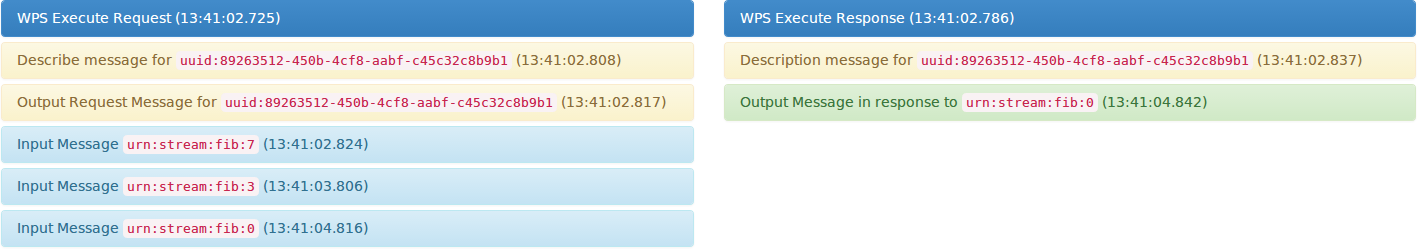
\includegraphics[width=\textwidth]{figures/fibonacci-1.png}
			\end{subfigure}
			\begin{subfigure}{\textwidth}
				\caption{$fib(1) = 1$ is supplied in an input message, and so the previously supplied request for $fib(2)$ and $fib(3)$ can be calculated. $fib(7)$ is still missing prerequisites.}
				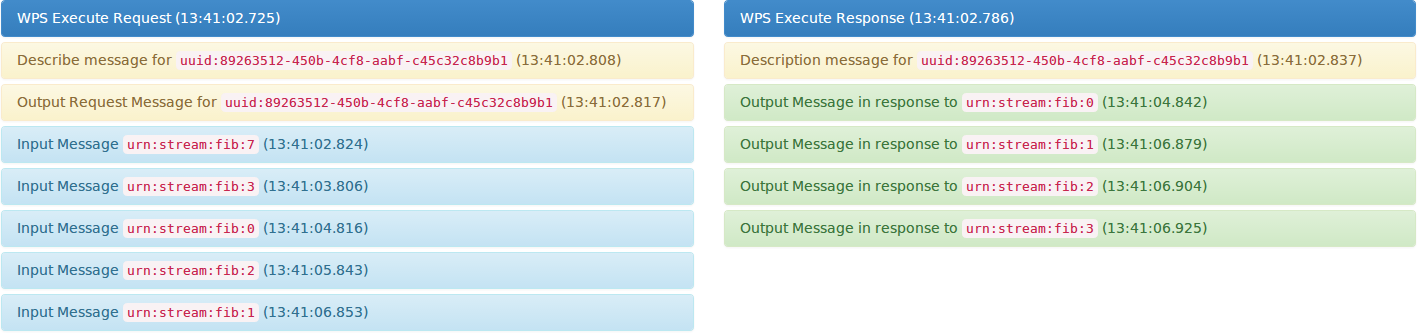
\includegraphics[width=\textwidth]{figures/fibonacci-2.png}
			\end{subfigure}
			\begin{subfigure}{\textwidth}
				\caption{As the dependencies of $fib(4)$ and $fib(5)$ are fulfilled, they can directly be calculated. $fib(7)$ is still missing the result of $fib(6)$.}
				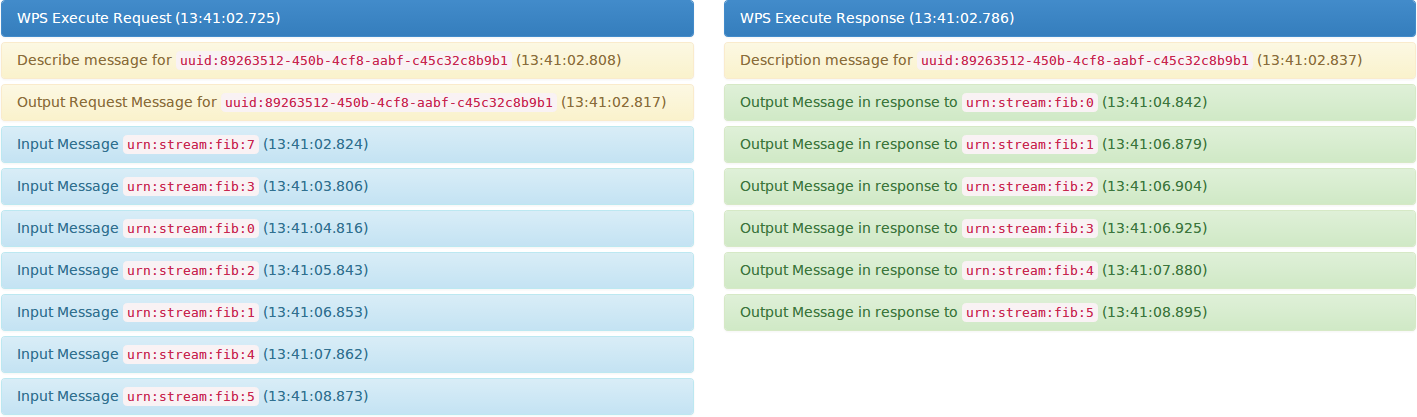
\includegraphics[width=\textwidth]{figures/fibonacci-3.png}
			\end{subfigure}
			\begin{subfigure}{\textwidth}
				\caption{At the time the request for $fib(6)$ arrives, all preconditions are met and $fib(6)$ and the final $fib(7)$ can be calculated. Once the result has arrived, the client stops the streaming process.}
				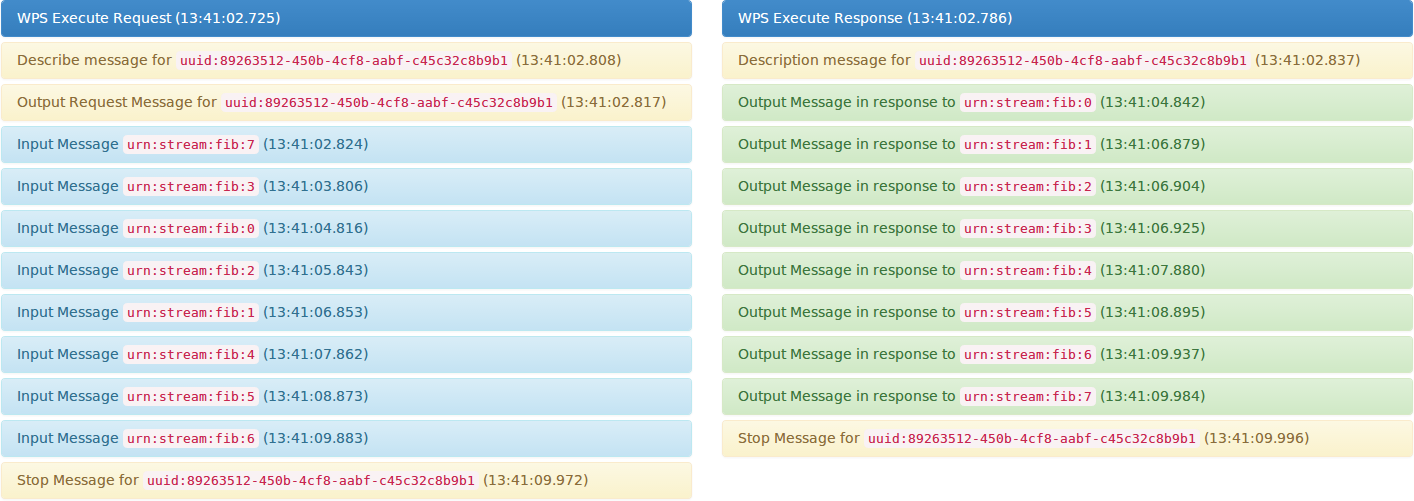
\includegraphics[width=\textwidth]{figures/fibonacci-4.png}
			\end{subfigure}
			\caption{\label{fig:client}Calculation of the seventh Fibonacci number using the Streaming WPS, its accompanying JavaScript API and a simple addition WPS process as the streaming process' delegate.}
		\end{figure}
	\section{Streaming \la WPS}
	\begin{itemize}
		\item simple application of the Streaming WPS and MATLAB WPS
		\item LakeAnalyzer may need further adjustments to allow live analysis
		\item remove down sampling code
		\item operate on single point in time
		\item etc
	\end{itemize}

\chapter{Discussion/Conclusion/Future Work}
	\begin{itemize}
		\item limitations of WPS standard
		\begin{itemize}
			\item different procedure description format, like in the SensorWeb
			\begin{itemize}
				\item differentiation between intermediate results and final result
				\item would make WPS standard less interoperable
			\end{itemize}
			\item process instance need to be identifiable
			\item WSDL like description language of WPS processes
			\begin{itemize}
				\item would allow specification of other transports
			\end{itemize}
			\item differentiation between continuous outputs and final results
			\item allow different transport layers (like WebSockets)
			\item allowing subsequent input parameters
		\end{itemize}
		\item MATLAB WPS future work
		\begin{itemize}
			\item extension to similar languages like octave
		\end{itemize}
		\item Streaming WPS future work
		\begin{itemize}
			\item No input/output conversion
			\item Only default format is requested from delegate
			\item process will not fail fast in under every condition
			\begin{itemize}
				\item inputs first are checked at execution time
			\end{itemize}
			\item receivers are only provided with upcoming outputs
			\begin{itemize}
				\item no replay queue
			\end{itemize}
		\end{itemize}
	\end{itemize}
